% ****** Start of file aipsamp.tex ******
%
%   This file is part of the AIP files in the AIP distribution for REVTeX 4.
%   Version 4.1 of REVTeX, October 2009
%
%   Copyright (c) 2009 American Institute of Physics.
%
%   See the AIP README file for restrictions and more information.
%
% TeX'ing this file requires that you have AMS-LaTeX 2.0 installed
% as well as the rest of the prerequisites for REVTeX 4.1
%
% It also requires running BibTeX. The commands are as follows:
%
%  1)  latex  aipsamp
%  2)  bibtex aipsamp
%  3)  latex  aipsamp
%  4)  latex  aipsamp
%
% Use this file as a source of example code for your aip document.
% Use the file aiptemplate.tex as a template for your document.
\documentclass[%
 aip,
%jmp,%
%bmf,%
%sd,%
rsi,%
 amsmath,amssymb,
%preprint,%
 reprint,%
%author-year,%
%author-numerical,%
]{revtex4-1}

\usepackage{graphicx}% Include figure files
\usepackage{dcolumn}% Align table columns on decimal point
\usepackage{bm}% bold math
%\usepackage[mathlines]{lineno}% Enable numbering of text and display math
%\linenumbers\relax % Commence numbering lines

\begin{document}

\preprint{AIP/123-QED}

\title[Sample title]{On the use of short reseeding trajectories to sample Markov state models}% Force line breaks with \\

% \author{A. Author}
%  \altaffiliation[Also at ]{Physics Department, XYZ University.}%Lines break automatically or can be forced with \\
% \author{B. Author}%
%  \email{Second.Author@institution.edu.}
% \affiliation{ 
% Authors' institution and/or address%\\This line break forced with \textbackslash\textbackslash
% }%

\author{Hongbin Wan}
\author{Vincent A. Voelz}
\email{vvoelz@temple.edu}
\affiliation{Department of Chemistry, Temple University, Philadelphia, PA 19122, USA}


\date{\today}% It is always \today, today,
             %  but any date may be explicitly specified

\begin{abstract}
In the last decade, advances in molecular dynamics (MD) and Markov State Model (MSM) methodologies have made possible accurate and efficient estimation of kinetic rates and reactive pathways for complex biomolecular dynamics occurring on slow timescales.  A promising approach to enhanced sampling of MSMs is to use so-called ?adaptive? methods, in which new MD trajectories are ?seeded? preferentially from previously identified states.  Here, we investigate the performance of various MSM estimators on reseeding trajectory, for both a simple 1D free energy landscape, and for mini-protein folding MSMs of WW domain and NTL9(1-39).  Our results reveal the practical challenges of reseeding simulations, and suggest a simple way to better estimate both thermodynamic and kinetic information.
\end{abstract}

\pacs{Valid PACS appear here}% PACS, the Physics and Astronomy
                             % Classification Scheme.
\keywords{kinetics, molecular simulation}%Use showkeys class option if keyword
                              %display desired
\maketitle

% \begin{quotation}
% The ``lead paragraph'' is encapsulated with the \LaTeX\ 
% \verb+quotation+ environment and is formatted as a single paragraph before the first section heading. 
% (The \verb+quotation+ environment reverts to its usual meaning after the first sectioning command.) 
% Note that numbered references are allowed in the lead paragraph.
% %
% The lead paragraph will only be found in an article being prepared for the journal \textit{Chaos}.
% \end{quotation}

\section{\label{sec:level1}Introduction}
In the last decade, Markov State Model (MSM) methodologies have made possible accurate and efficient estimation of kinetic rates and reactive pathways for slow and complex biomolecular dynamics.\cite{Noe:2009en,Voelz:2010hs,Prinz:2011id,Chodera:2014gk,noe2014introduction} One of the key advantages touted by MSM methods is the ability to use large ensembles of short-timescale trajectories for sampling events that occur on slow timescales.  The main idea is that sufficient sampling using many short trajectories can circumvent the need to sample long trajectories.

With this in mind, many ``adaptive'' methods have been developed for the purpose of accelerating sampling of MSMs.  The simplest of these can be called \textit{adaptive seeding}, where one or more new rounds of unbiased simulation are performed by ''seeding'' swarms of trajectories throughout the landscape.\cite{Huang:2009bx} The choice of seeds are based on some initial approximation of the free energy landscape, possibly from non-equilibrium or enhanced-sampling methods.  Adaptive seeding can be performed by first identifying a set of metastable states, then initiating simulations from each state.  If the seeding trajectories provide sufficient connectivity and statistical sampling of transition rates, an MSM can be constructed to accurately estimate both kinetics and thermodynamics.  
 
Similarly, so-called \textit{adaptive sampling} algorithms have been developed for MSMs in which successive rounds of targeted seeding are performed, updating the MSM after each round\cite{Voelz:2014kk,Shamsi:2017jg}. A simple adaptive sampling strategy is to start successive rounds of simulations from under-sampled states, for instance, from the state with the least number of transition counts.\cite{Doerr:2014fc}  A more sophisticated approach is the FAST algorithm, which is designed to discover states and reactive pathways of interest by choosing new states based on an objective function that balances under-sampling with a reward for sampling desired structural observables.\cite{Zimmerman:2015kf,Zimmerman:2018jn} The REAP algorithm efficiently explores folding landscapes by using reinforcement learning to choose new states.\cite{shamsi2017reinforcement}

A key problem with adaptive sampling of MSMs arises because we are often interested in \textit{equilibrium} properties, while trajectory seeding is decidedly \textit{non-equilibrium}.  This may seem like a subtle point, because the dynamical trajectories themselves are unbiased, but of course, the ensemble of starting points for each trajectory are almost always \textit{statistically} biased, i.e. the seeds are not drawn from the true equilibrium distribution.  This can problematic because most MSMs are constructed from transition rate estimators that enforce detailed balance and assume trajectory data is obtained at equilibrium. The distribution of sampled transitions, however, will only reflect equilibrium conditions in the limit of long trajectory length.

One way around this is to focus mostly on the kinetic information obtained by adaptive sampling.  A recent study of the ability of FAST to accurately describe reactive pathways concluded that the most reliable MSM estimator to use with adaptive sampling data is a row-normalized transition count matrix.\cite{Zimmerman:2018jn} Indeed, weighted-ensemble path sampling algorithms focus solely on sampling the kinetics of reactive pathways, information which can be used to recover global thermodynamic properties.\cite{BinWZhang:2010kf,Zwier:2015fn, Dickson:2016it, Lotz:2018hx, Dixon:2018fs} A major disadvantage of this approach is that it ignores potentially valuable equilibrium information.  As shown by Trendelkamp-Schroer and No{\'e},\cite{trendelkamp2016efficient} detailed balance is a powerful constraint to infer rare-event transition rates from equilibrium populations.  Specifically, when faced with limited sampling, dedicating half of one's simulation samples toward enhanced thermodynamic sampling (e.g. umbrella sampling) can result in a significant reduction in the uncertainty of estimated rates, simply because the improved estimates of equilibrium state populations inform the rate estimates through detailed balance.

Another way around this problem, recently described by N{\"u}ske et al., is to use an estimator based on observer operator model (OOM) theory which utilizes information from transitions observed at lag times $\tau$ and $2\tau$ to obtain estimates unbiased by the initial distribution of seeding trajectories.\cite{Nuske:2017ex}  Although the OOM estimator is able to make better MSM estimates at shorter lag times, it requires the storage of a transition count array that scales as $\propto N^3$ for a MSM with $M$ states, and a dense-matrix singular-value decomposition step, which may make it impractical for MSMs with large numbers of states.  N{\"u}ske et al. derive an expression quantifying the error incurred by non-equilibrium seeding, from which they conclude that such bias is difficult to remove without either increasing the lag time or improving the state discretization.  Both strategies are antithetical to adaptive seeding, the purpose of which is to utilize swarms of very short trajectories from previously-defined MSM states. 

In this manuscript, we explore an alternative way to recover accurate MSM estimates from biased seeding trajectories, by \textit{reweighting} the sampled transitions counts to better approximate counts that would be observed at equilibrium.  Like the Trendelkamp-Schroer and No{\'e} method, this requires some initial estimate of state populations, perhaps obtained from previous rounds of adaptive sampling.

Moreoever, we are particularly interested in examining how our reweighting method performs in cases where it is impractical to generate long trajectories and instead are forced to rely on ensembles of short seeding trajectories. An example of this is adaptive seeding of protein folding MSMs built from ultra-long trajectories simulated on the Anton supercomputer\cite{DESRES}  Because such computation is not a widely available resource, adaptive seeding using more conventional computers may be one of the only ways to leverage these MSMs to predict the effect of mutations, for example. 

Here, 
In this manuscript, we make the case that even the most basic kind of adaptive sampling, i.e. single-round \textit{adaptive seeding}, benefits from MSM estimates that include equilibrium population estimates.  We first show this in a simple 1-D model, and then show its application in a practical scenario: adaptive seeding of protein folding MSMs using large-scale distributed computing. Our results suggest a simple method to make reseeding simulations more accurate. Finally we apply the method to predict mutation induced kinetics. The overall results indicate the wide ranging applicability from doing proper estimations in seeding simulations to predict perturbed kinetics. 

\subsection{\label{sec:level2}Adaptive seeding of folding landscapes}

To character of the protein folding landscapes remains the challenging in molecular biology even using GPU-acceleration or simulation on the \textit{Anton}, special-purpose supercomputer) due to the rough and large energy barriers. On the other hand, there are great interests in using molecular dynamics simulations along with MSM methodologies, which can offer a seemingly simple way to improve the conformational sampling efficiency for obtaining the full folding/unfolding behaviors.\cite{Voelz:2014kk,Shamsi:2017jg,Zimmerman:2018jn} In concept, MSMs should guide the simulations to explore conformational spaces. Based on this idea that motivates the recent development of multiensemble Markov model \textbf{MEMM}, which applies transition-based reweighting method to properly estimate MSMs simulated with bias/un-bias.\cite{Wu:2016fk} It should be noted that it is unlike Weighted-ensemble (WE) path sampling algorithms, which can also be classified as adaptive sampling algorithms. In WE approaches such as WExplore\cite{Dickson:2014du} and WESTPA\cite{Zwier:2015fn}, successive rounds of new trajectories are spawned to better sample a quantity of interest (reactive flux, for example), while the statistical weights of each trajectory are carefully managed so that no bias is introduced. The above adaptive methods are unbiased, where the bias here are in the sense that each trajectory is simulated with changed potential/pre-defined reaction coordinates. This statistical bias has interesting consequences in estimating various quantities, consequences which arise from the trade-off between sampling of transition rates versus equilibrium probabilities.  Thus, the adaptive seeding simulations need an proper estimator instead of the maximum-likelihood estimator (MLE) that is default in packages like MSMBuilder.\cite{Pande:2010ik,Prinz:2011id,McGibbon:2015fv,Kellogg:2012cu,Metzner:2009jx,Nuske:2014kk} This is because the MLE enforces detailed balance; i.e. MLE assumes that the observed counts are sampled from the equilibrium distribution, an assumption which is (purposely) violated by adaptive sampling.  One might expect, then, that while quantities like rates and pathways are accurately estimated by adaptive methods, quantities like equilibrium populations may have more uncertainties and/or bias.  Indeed, while the weighted ensemble algorithms have recently been used to efficiently sample very slow folding rates \cite{Dickson:2016it} ad unbinding rates (residence times $>$ 10 s), these same algorithms(.....???? need to edit)

In this paper, we consider a specific kind of adaptive method for sampling MSMs: adaptive seeding of perturbed folding landscapes.  It is often the case that large numbers of expensive simulations in a particular force field are utilized to model the folding landscape of a particular protein sequence. We would like to model the folding of a sequence variant, or perhaps use a different force field potential, without having to perform a heroic amount of simulation.  Since there is much prior information from the \textit{wild-type} MSM, it is reasonable to think that adaptive seeding could provide a good picture of how folding rates and populations change with the perturbation.  Here, we explore the accuracy of several estimators for obtaining folding rates and populations from adaptive seeding simulations.  
Using a 1-D two-state potential as simple model, we explore different estimators and find interesting differences in their relative accuracies in estimating rates versus equilibrium populations from adaptive seeding trajectory data.  We also explore  the effects of using different trajectory lengths and number of seeds. In general, we find that rates and free energies are more accurately estimated by estimators that incorporate some prior knowledge of the equilibrium populations. We then show how adaptive seeding can be used to model changes in folding rates and populations for GTT WW domain and K12M mutant of NTL9, based on MSMs built from ultra-long simulation trajectories.


\subsection{\label{sec:level2}Estimators}

We explored the accuracy and efficiency of several different transition probability estimators using the adaptive seeding trajectory data as input: (1) a maximum-likelihood estimator (MLE), (2) a MLE estimator where the equilibrium populations $\pi_i$ of each state are known \textit{a priori}, (3) the MLE estimator where each input trajectory is weighted by the \textit{a priori} equilibrium population of its starting point,(4) row-normalized transition counts and (5) Observable operator model estimators.

\subsubsection{Maximum-likelihood estimator (MLE).} 
The MLE for a reversible MSM assumes that observed transition counts are independent, and drawn from the equilibrium distribution, so that reversibility (i.e. detailed balance) can be used a constraint.  The likelihood of observing a set of given transition counts, $L = \prod_i \prod_j p_{ij}^{c_{ij}}$, when minimized under the constraint that $\pi_i p_{ij} = \pi_j p_{ji}$, for all $i, j$, yields a self-consistent expression that can be iterated to find the equilibrium populations,\cite{Wu:2014jya, Prinz:2011id, Bowman:2009jw}
\begin{equation}
\pi_i  = \sum_j \frac{c_{ij} + c_{ji}}{\frac{N_j}{\pi_j} + \frac{N_i}{\pi_i}}
\end{equation}
where $N_i = \sum_j c_{ij}$.  The transition probabilities $p_{ij}$ are  given by 
\begin{equation}
p_{ij} = \frac{(c_{ij} + c_{ji})\pi_j }{N_j\pi_i + N_i\pi_j } 
\end{equation}

\subsubsection{Maximum-likelihood estimator (MLE) with known populations $\pi_i$}
Minimization of the likelihood function above, with the additional constraint of fixed populations $\pi_i$, yields a similar self-consistent equation that can be used to determine a set of Lagrange multipliers,\cite{TrendelkampSchroer:2016bz}
\begin{equation}
\lambda_i  = \sum_j \frac{(c_{ij} + c_{ji})\pi_j \lambda_i}{\lambda_j\pi_i + \lambda_i\pi_j },
\end{equation}
from which the transition probabilities $p_{ij}$ can be obtained as
\begin{equation}
p_{ij} = \frac{(c_{ij} + c_{ji})\pi_j }{\lambda_j\pi_i + \lambda_i\pi_j }.
\end{equation}

\subsubsection{Maximum-likelihood estimator (MLE) with population-weighted trajectory counts.}
For this estimator, first a modified count matrix $c_{ij}'$ is calculated, 
\begin{equation}
c_{ij}' = \sum_k w^{(k)}c_{ji}^{(k)},
\end{equation}

where transition counts $c_{ji}^{(k)}$ from trajectory $k$ are weighted in proportion to $w^{(k)} = \pi^{(k)}$, the equilibrium population of the initial state of the trajectory.  The idea behind this approach is to counteract the statistical bias from adaptive seeding by scaling the observed transition counts proportional to their equilibrium fluxes.The modified counts are then used as input to the MLE.

\subsubsection{Row-normalized counts.}
For this estimator, the transition probabilities are approximated as
\begin{equation}
p_{ij} = \frac{c_{ij}}{\sum_j c_{ij}}.
\end{equation}
This approach does not guarantee reversible transition probabilities, which only occurs in the limit of large numbers of reversible transition counts.  In practice, however, the largest eigenvectors of the transition probability matrix have very nearly real eigenvalues, such that we can report relevant relaxation timescales and equilibrium populations. 

\subsubsection{Observable operator model(OOM) theory}
For this estimator, it requires count matrix $C_{Eq}^{\tau}$ and two-step count matrix $C_{Eq}^{2\tau}$ to obtain the unbiased equilibrium correction matrix and unbiased equilibrium distribution.\cite{Nuske:2017ex} The non-reversible and reversible transition probabilities are approximated as
\begin{equation}
T_{Eq}^{\tau}(i,j)=\frac{C_{Eq}^{\tau}(i,j)}{\pi_{i}}
\end{equation}

\begin{equation}
T_{Eq}^{\tau}(i,j)=\frac{T_{Eq}^{\tau}(i,j)+T_{Eq}^{\tau}(j,i)}{\sum_{j=1}^{N}T_{Eq}^{\tau}(i,j)+\sum_{j=1}^{N}T_{Eq}^{\tau}(j,i)}
\end{equation}

This approach does not only correct MSM estimates with a shorter lag times but also can play an indicator of the equality from of such MSMs. However, the computational cost of this estimator is heavy, which is proportional to $N^{3}$ (N is the number of MSM states) for example.   

%%%%% wide figure
\begin{figure*}
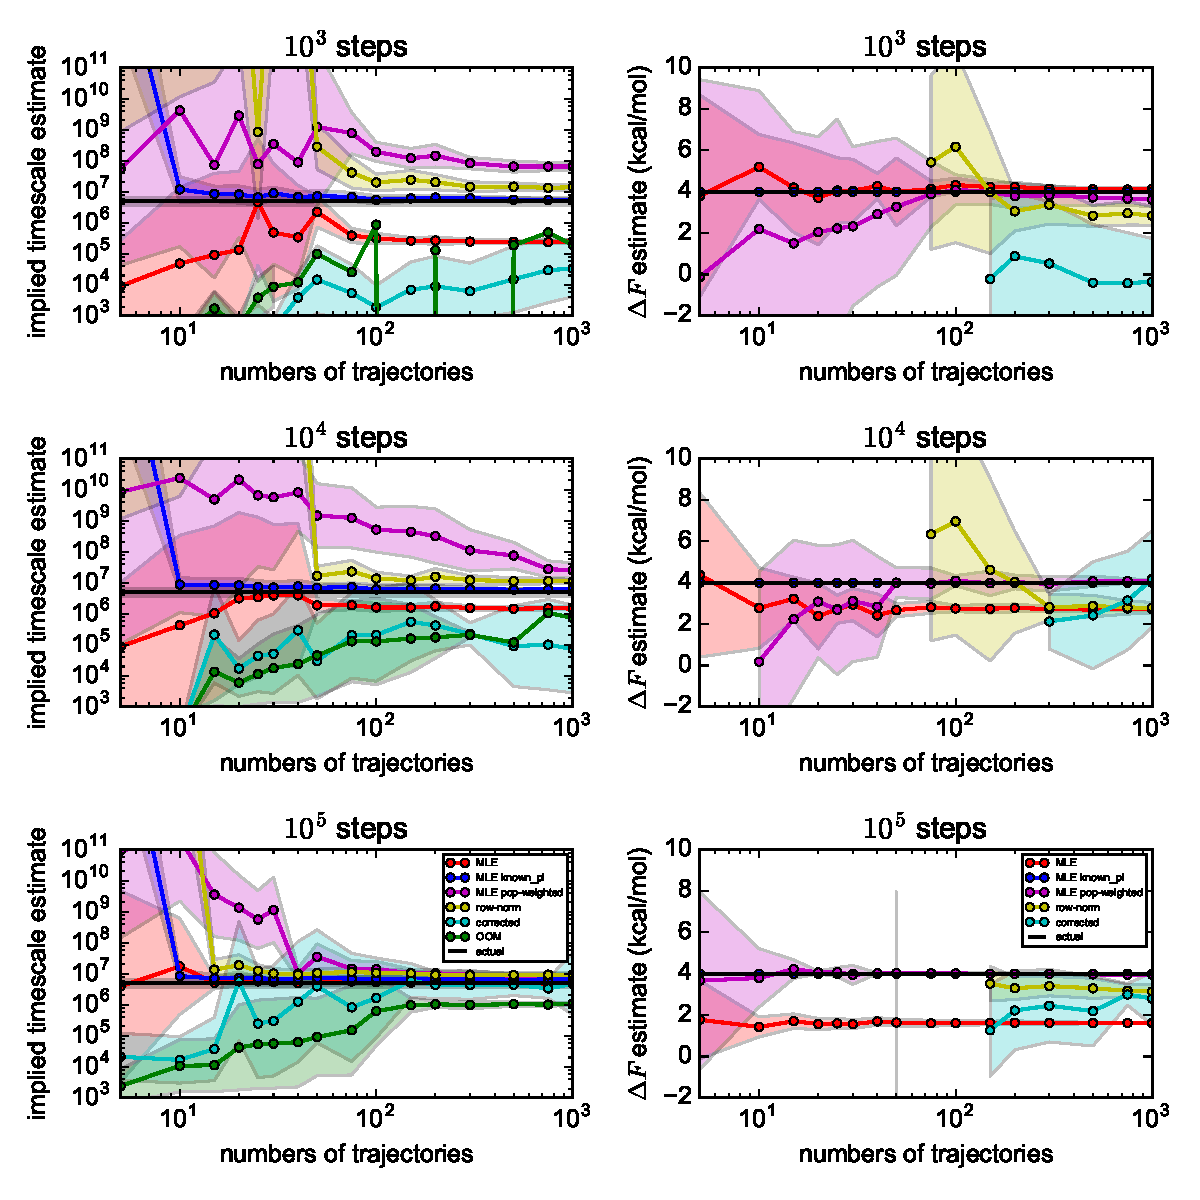
\includegraphics[width=1.5\columnwidth]{figures/convergence_oct2018.pdf}% Here is how to import EPS art
\caption{\label{fig:wide}The performances on predictions of implied timescales and free energy from different estimators}
\end{figure*}

\section{Results}

\subsection{Adaptive seeding of a 1-D potential energy surface}

We consider the following potential energy surface, as used by Stelzl et al.\cite{Stelzl:2017gra}:  $U(x) = -\frac{2k_BT}{0.596} \ln [ e^{-2(x-2)^2-2} + e^{-2(x-5)^2} ] $
for $x \in [1.5,5.5]$, and $k_BT = 0.596$ kcal mol$^{-1}$.  The state space is uniformly divided into 20 bins to calculate discrete-state quantities. Diffusion on the 1-D landscape is approximated by a Markov Chain Monte Carlo (MCMC) procedure in which new moves are translations randomly chosen from $\delta \in [-0.05, +0.05]$ and accepted with probability $\min(1, \exp( \beta [U(x+\delta)-U(x)]))$, i.e. the Metropolis criterion.

\begin{figure}[ht!]
    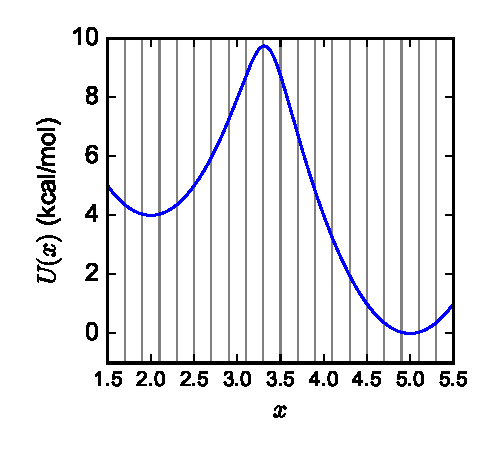
\includegraphics[width=0.9\columnwidth]{figures/1D-potential}
    \caption{A 1-D two-state potential}.
    \label{fig:1D-potential}
\end{figure}

For all tests with this toy model, we limit the lag time to $\tau =$ 100 steps.  To estimate the ''true'' relaxation timescale of the two-state model, we generated long MCMC trajectories of $10^9$ steps, sampling from a series of scaled potentials $U^{(\lambda)}(x) = \lambda U(x)$ for $\lambda \in [0.5, 0.6, 0.7, 0.8, 0.9, 1.0]$. For each $\lambda$ value, 20 trajectories were generated, with half of them starting from $x=2.0$ and the other half starting from $x=5.0$, resulting in a total of 120 trajectories.  The DTRAM estimator of Wu et al.\cite{Wu:2014jy} was used to estimate the slowest relaxation timescale as 9.66 ($\pm$ 1.37) $\times 10^6$ steps, using a lag time of 1000 steps.

To emulate adaptive seeding trajectory data, various numbers of trajectories $s$, each of length $n\tau$ were initiated from the center positions of all twenty bins.  The resulting data consists of $20 \times s \times n$ transition counts between states $i$ and $j$ in lag time $\tau$, stored in a 20 $\times$ 20 count matrix of entries $c_{ij}$.  From these counts, estimates of the transition probabilities, $p_{ij}$ can be made. The MLE with known populations undoubtedly gets converged on the predictions of  both implied timescales and free energy profiles due to only 1 reaction coordinate defined in the simulations. The Maximum Likelihood estimator(MLE) requires longer simulations to get accurate implied timescale estimations and OOM estimator always underestimates the implied timescale. As expected, the row normalization estimator is hard to work with large lagtime in these short seeding simulations. With population-weighted trajectory counts,Maximum-likelihood estimator(MLE) reaches the right implied timescale very fast if the trajectory length is long or more seeding trajectories ware simulated. Interestingly, MLE successfully captures the right free energy profile with short simulations but starts to lose performances in longer seeding simulations. The free energy profile estimated from OOM starts to become better if more trajectories data can be collected. The population-weighted MLE gets converged very fast on predicting the free energy profile even with short seeding simulation length or smaller number of simulations trajectories.       

\subsection{Seeding of folding landscapes for WW Domain and NTL9(1-39)}

The WW domain, one of the fast-folding protein domains, is 35-residue proline-rich protein that consists of three $\beta$-sheet structure, whose kinetics has been extensively studied by experiments\cite{Nguyen:2003gw,Jager:2006ga,Liu:2008fs,Dave:2016joa,Liu:2008kj}. And it also has been characterized to be a benchmark system in molecular dynamics to explore two-state fast-folding behaviors and downhill folding manners\cite{Gao:2017kna,Best:2013hua,Piana:2011gma}. A large number of mutation experiments have been done to investigate its folding mechanisms. Among the variants of its families,a WW domain of the FIP mutant(FiP35) of protein human pin1 has a folding time of 13$\mu$s\cite{HoubiNguyen:2005ec}. Another optimization near loop2 where native sequence Asn-Ala-Ser (NAS) is replaced with Gly-Thr-Thr(GTT) tri-mutations was discovered by Piana et al. that has a fast relaxation time ~4 $\mu$s\cite{Piana:2011gma}. Two independent ultra-long trajectories(651 and 486 $\mu$s) provided by Shaw et al.\cite{LindorffLarsen:2011gla} were performed at 360K using the CHARMM22* force field.

NTL9(1-39) domain is the N-terminal domain of the ribosomal protein L9, and its folded state consists of one $\alpha$-helix and three-strand $\beta$-sheet. NTL9 domain is widely used as a classic system to study  two-state folders in both experimental and computational studies\cite{Cho:2004dp,Cho:2005is,Voelz:2010hsa,Hoffman:1994hk,Schwantes:2013bpa}. The K12M mutant in the hydrophobic core destabilizes the non-native states and has a faster folding rate\cite{Cho:2014fla}. The K12M mutant of NTL9(1-39) trajectories provided by Shaw et al. were four MD simulations of 1052$\mu$s, 990$\mu$s, 389$\mu$s, and 377$\mu$s at 355K with CHARMM22* force field\cite{LindorffLarsen:2011gla}.

\subsubsection{Markov State Model construction}

The MSM of the GTT WW domain at 360K was previously descried by Wan\cite{WAN:2016fz}, which used eight tICA components and a lag time of 10ns to find the best low dimensional subspace. A 1000 micro-state MSM with a lag time 100ns using k-center clustering,which was determined by GMRQ method,\cite{McGibbon:2015gm} to best capture its folding behaviors. The relaxation time scales of 10.2$\mu$s was estimated from MSM, which was well matched to a folding time 21 � 6$\mu$s predicted by Shaw\cite{LindorffLarsen:2011gla} and 8$\mu$s for a three-state model of GTT folding by Beauchamp\cite{Beauchamp:2012kp}. As a better test of different estimating approaches due to large timing used in OOM analysis, we built a 200 micro-state MSM which showed 2.3$\mu$s folding time. 

The MSM of the K12M mutant of NTL9(1-39) was previously described by  Schwantes and Lin\cite{Schwantes:2013bpa,Baiz:2014gm,Beauchamp:2012kp}. A folding time 18$\mu$s was observed from the MSMs and the 6 components was chosen as input for tICA metric to best project trajectories on low-dimensional subspace. The optimal lagtime 200ns and 1000 micro-states, determined by GMRQ\cite{McGibbon:2015gma}, were used to accurately capturing folding dynamics of NTL9(1-39). A relaxation time ~18$\mu$s was observed, compares well to 29$\mu$s predicted by Shaw\cite{LindorffLarsen:2011gla} and to the folding rate of 26.4 $\mu$s (at 80$\,^{\circ}\mathrm{C}$), obtained from the T-jump experiments\cite{Baiz:2014gm}. Similarly to GTT system, we built a 200 micro-state MSM for a better comparison using didfferent estimators, which showed 5.2$\mu$s folding time.

Reseeding simulations trajectories  starting from each micro-state of both GTT and NTL9 system were randomly picked from these MSMs built from these two ultra-large data-sets($\sim$1.1ms for GTT and $\sim$ 2.8ms for NTL9). Totally, 12 and 14 reversible folding behaviors were observed for GTT and NTL9 in these two data-sets respectively\cite{LindorffLarsen:2011gla}. We believe that random seeded simulations trajectories from these two data-sets are amenable to explore the effects of reseeding methods. To test the effects from reseeding numbers of trajectories and lengths of trajectories, several rounds of analysis were managed to construct the reseeding simulation trajectories. We collected 5 and 10 reseeding trajectories starting from all micro states with different lengths from both 200 micro-state and 1000 micro-state models and explored the performances of different estimators. The sizes of cumulative seeding trajectories for each MSM were chosen to be less than original ultra-large data-sets.

The equilibrium populations used to do population re-weighting estimation and known population estimation were predicted from MSMs. And notably, Row-normalized estimator could not work with large lagtime in short seeding trajectories, thus, we added the minimum counts to each element in count matrices to avoid getting un-representable values in division calculations. We are expecting a faster folding rate estimation and a more evenly distributed population estimation. 

\subsubsection{Predictions of Folding Rates from reseeding trajectories with different estimators}

%%%%% wide figure
\begin{figure*}
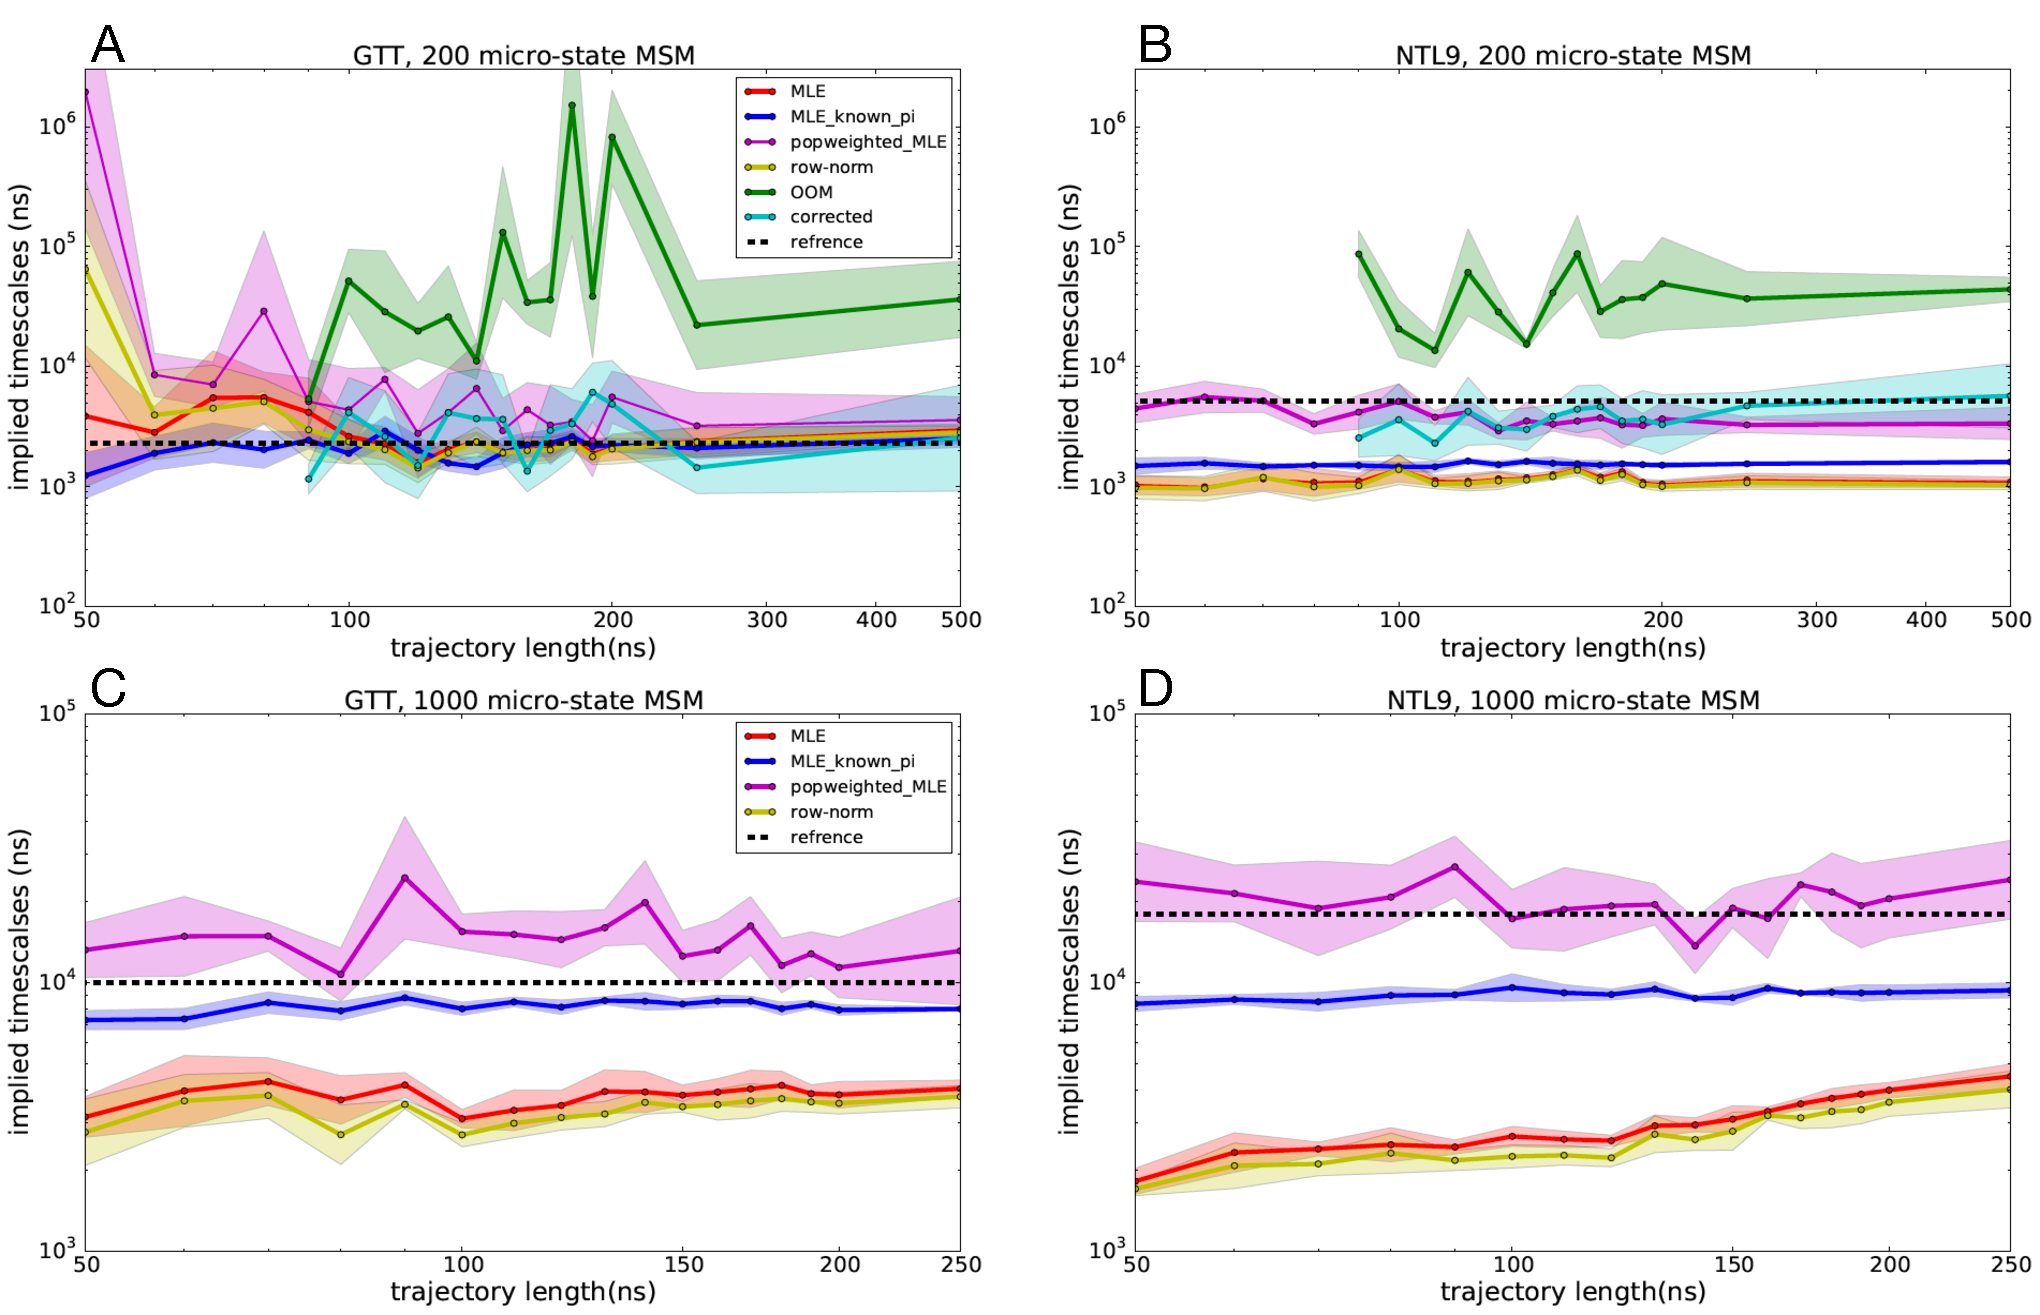
\includegraphics[width=0.8\paperwidth]{figures/Slowest_timescales_only/all_slowest_timescales_cluster_200_and_1000_omi.pdf}
\caption{((a)and(b)) are the estimates for the slowest relaxation time scales from different estimators on the 200-microstate MSMs of GTT(left) and NTL9(right).((c)and(d)) are the estimates for the slowest relaxation time scales from different estimators on the 1000 micro-state MSMs of GTT(left) and NTL9(right).}
\end{figure*}


Given that our references 200 and 1000 micro-state MSMs predicted the GTT WW domain and NTL9 have folding time at 2.3, 10.2\cite{WAN:2016fz} and 5.2, 18 $\mu$s\cite{Schwantes:2013bpa,Baiz:2014gm} respectively. We then applied different estimator approaches to our reseeding trajectories to predict both kinetics and thermodynamics of each system. The computed folding relaxation time scales from MLE estimator for these 200 micro-state MSMs built from 5 independent seeding trajectories starting from each micro state are within tolerance but way off for 1000 micro-state MSMs, even we extended all the trajectories length from 50ns to 250ns in 1000 micro-state MSMs, which still failed to improve the time scales estimations. We then examined the performance of MLE estimator with 10 independent seeding trajectories form each state, and again MLE inaccurately predicted all relaxation timescales(SI). 

The folding time scales of GTT and NTL9 predicted with Maximum Likelihood estimator(MLE) with known populations successfully rescued the poor performances with MLE estimator, which yield really closed folding rates comparing to the references. Importantly, we note that the rate estimations do not rely on the length of trajectories.This is of course a huge advantage in doing seeding simulations which would reduce the computational time. We also find that 5 seeding trajectories suffering minimally comparing to more seeding trajectories(SI). However, only native state population was known at most time ahead of simulations,which limited the usages with this estimator in common model-builds.

With population-weighted trajectory counts, Maximum-likelihood estimator (MLE) correctly rescued the relaxation time estimations in both 200 and 1000 micro-state MSMs. Amazingly, we note that this estimator does not depend on the length of trajectories. The data size needed to accurately capture the right folding time is much smaller than the original data-sets, which reduces the computational time a lot. More importantly, this estimator is more applicable on predicting the effects from perturbations including mutations, temperatures and different force-fields if a well-defined MSM was provided ahead.

Row-normalized counts estimator can only work if the connectivity between states is not zero, however it is tough to be approached with a larger lag time in short seeding simulations. The performances in both GTT and NTL9 systems were so poor because of the poor connectivity, even with the pseudo counts added to purposely make this estimator work. However, it is a mathematical solution in a long seeding simulations, which is against the purpose of doing short seeding simulations. 

The OOM framework with bootstrapping count metric only works with longer seeding simulations, which ensures the connectivity between the pair-wised states. And the OOM overestimates the relaxation timescales in both GTT and NTL9 systems, while the corrected MSMs estimate time scales are one magnitude smaller and closely capture the referenced range. Furthermore, the practical application of OOM methods are limited by the number of states, simply due to the $(N^3)$  scaling of the algorithm limits the calculation for the all-atom models to 200 states.

\subsubsection{Predictions of native-state population from reseeding trajectories with different estimators}

Both GTT and NTL9 were two classical two-state folder systems from extensively studied. The accuracies of native state population estimations are expected to closely match to the predictions on the kinetics because of the expected single energy barrier in these two systems. The analysis above showed MLE with known populations estimator could accurately capture the slowest relaxation time,thus the native state population was expected to be well estimated, which is always true in this case.  The row-normalized counts estimator all had a fast folding rate for both GTT and NTL9 systems, which indicated these estimators inaccurately predicted a flatter energy barriers for these two-state folders. Notably, row-normalized counts estimator wrongly predicted a small native-state population due to the pseudo counts, which made the folding landscape even flatter in this 1000 micro-state model. The MLE estimator underestimated the native state population in both 200 and 1000 micro-state models. The MLE with population-weighted trajectory counts estimator successfully capture the the native-state population in 200 micro-state model but a little over estimated the native state population in 1000 micro-state models, however, the estimation got better with longer seeding simulations. Furthermore, The data-set needed to get a converged population estimation with population-weighted MLE is much smaller than the other estimators. The OOM poorly estimated the population of the native state in both GTT and NTL9 systems and the estimates were independent on the the trajectory length, where it may be resulted from bad state discretization or much longer seeding simulations trajectories are needed for the application of this method.

\begin{figure*}
\includegraphics[width=0.8\paperwidth]{figures/NTL9_GTT/native_state_population_only/native_population_5trajs_cluster200_1000_omi.pdf}% Here is how to import EPS art
\caption{The native state population estimations of both GTT((a) and (c)) and NTL9((b) and (d)) with different estimators from 200 and 1000 micro-state MSMs.}
\end{figure*}


\subsubsection{Predictions of mutation effect from reseeding trajectories with different estimators}

As a further test of the Maximum-likelihood estimator (MLE) with population-weighted trajectory counts estimator in predicting perturbation effects, several more MSMs were built from seeding trajectories of GTT and FiP35 from four additional GTT simulations trajectories(83, 118, 124, and 272 $\mu$s)\cite{HoubiNguyen:2005ec,Piana:2011gma} with and six ?100 $\mu$s FiP35 simulations trajectories with AMBER ff99SB-ildn force field at 395K\cite{Shaw:2010ge,Piana:2011gma}.As a fast folding sequence, FiP35 has a folding time of 13$\mu$s which is slower than GTT mutant\cite{Nguyen:2005ec}. 

The results in 200 micro-state model for both GTT and FiP35, OOM overestimated the folding times and all the other estimators undereatimated the folding time. However, it is amazingly that population-weighted trajectory counts estimator closely captured the folding time for both GTT and FiP35. And population-weighted estimator were the best to predict the native-state populations always. Notably, population-weighted estimator did not successfully predict the folding time and notabilities resulted in mutation effects, but we assume it may be caused by finite sampling errors, however, the population-weighted estimator was independent on seeding trajectory length in both systems, which raised our interests about how robust that this estimator can work in predicting  the larger perturbations of landscape from mutations, force fields, temperature etc.

\begin{figure*}
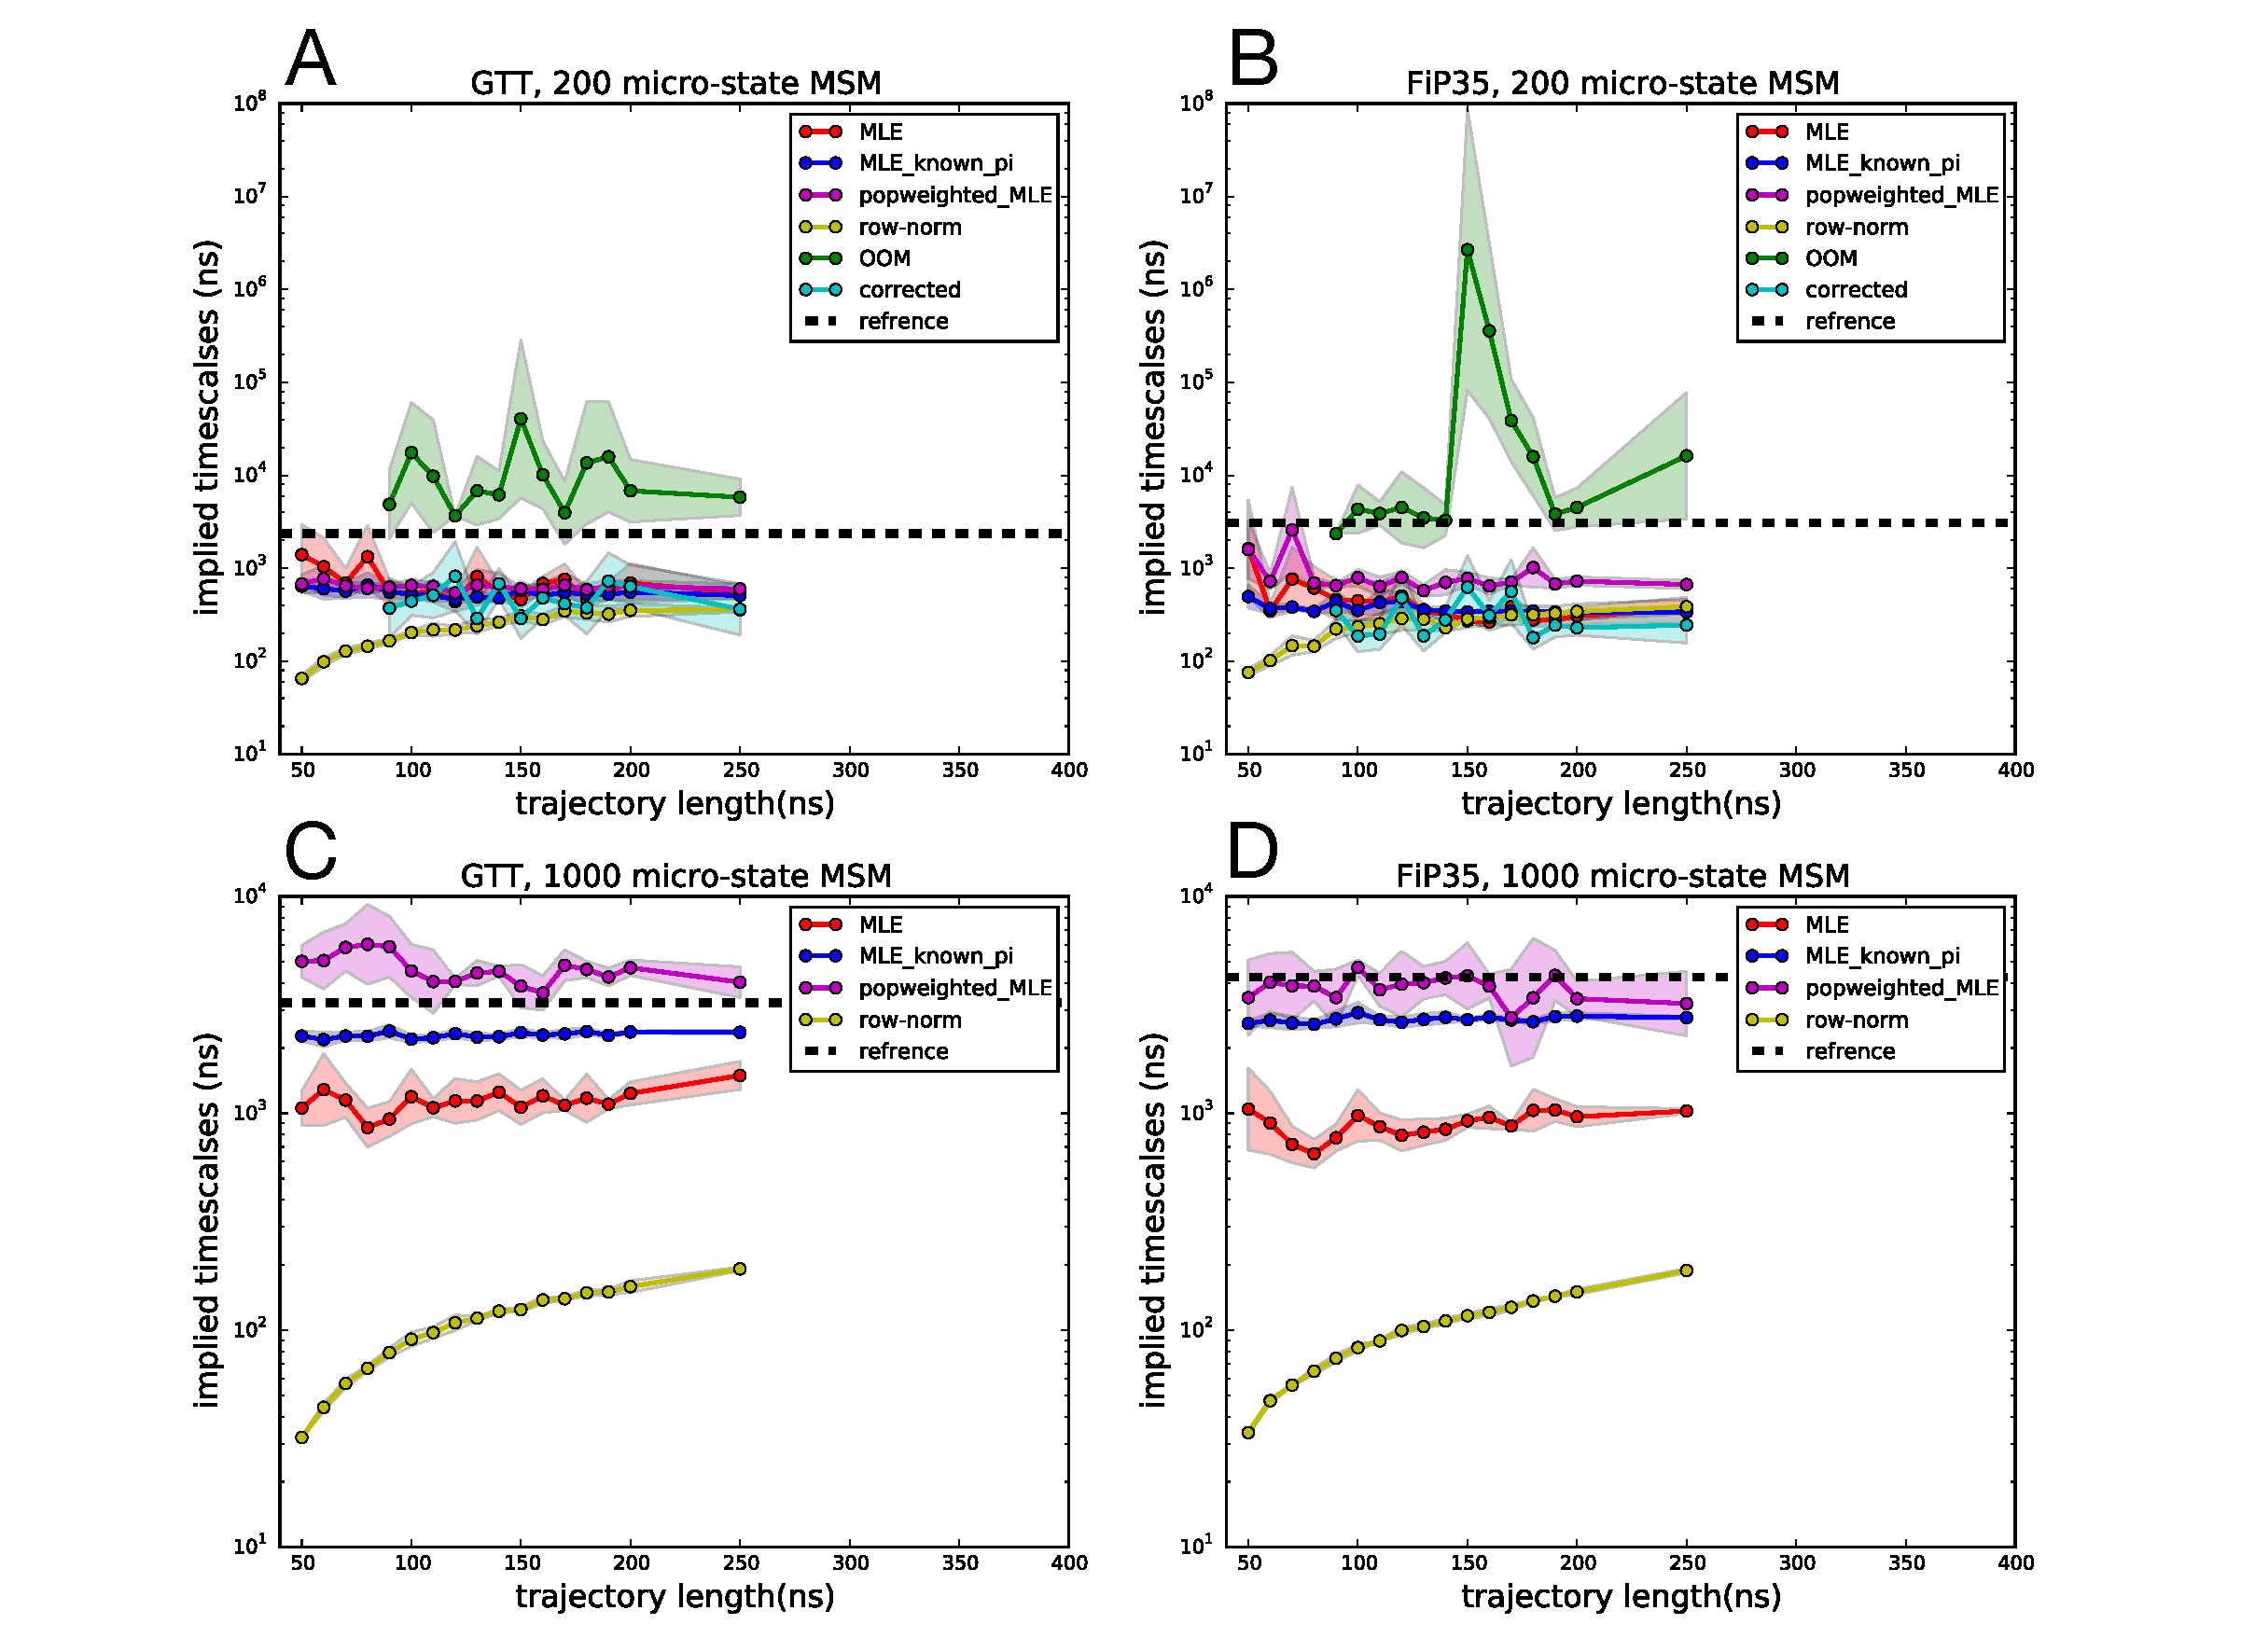
\includegraphics[width=0.8\paperwidth]{figures/Slowest_timescales_only/GTT_FiP35_ipt.pdf}% Here is how to import EPS art
\caption{Maximum-likelihood estimator (MLE) with population-weighted trajectory counts estimator for FiP35(right) and MLE estimator for GTT (left) show FiP35 folds slower than GTT}
\end{figure*}

\begin{figure*}
\includegraphics[width=0.8\paperwidth]{figures/NTL9_GTT/native_state_population_only/GTT_FIP35_395K_native_population_5trajs_cluster200_and_1000_omi.pdf}% Here is how to import EPS art
\caption{The native state population estimations of both GTT((a) and (c)) and NTL9((b) and (d)) with different estimators from 200 and 1000 micro-state MSMs.}
\end{figure*}

\begin{figure*}
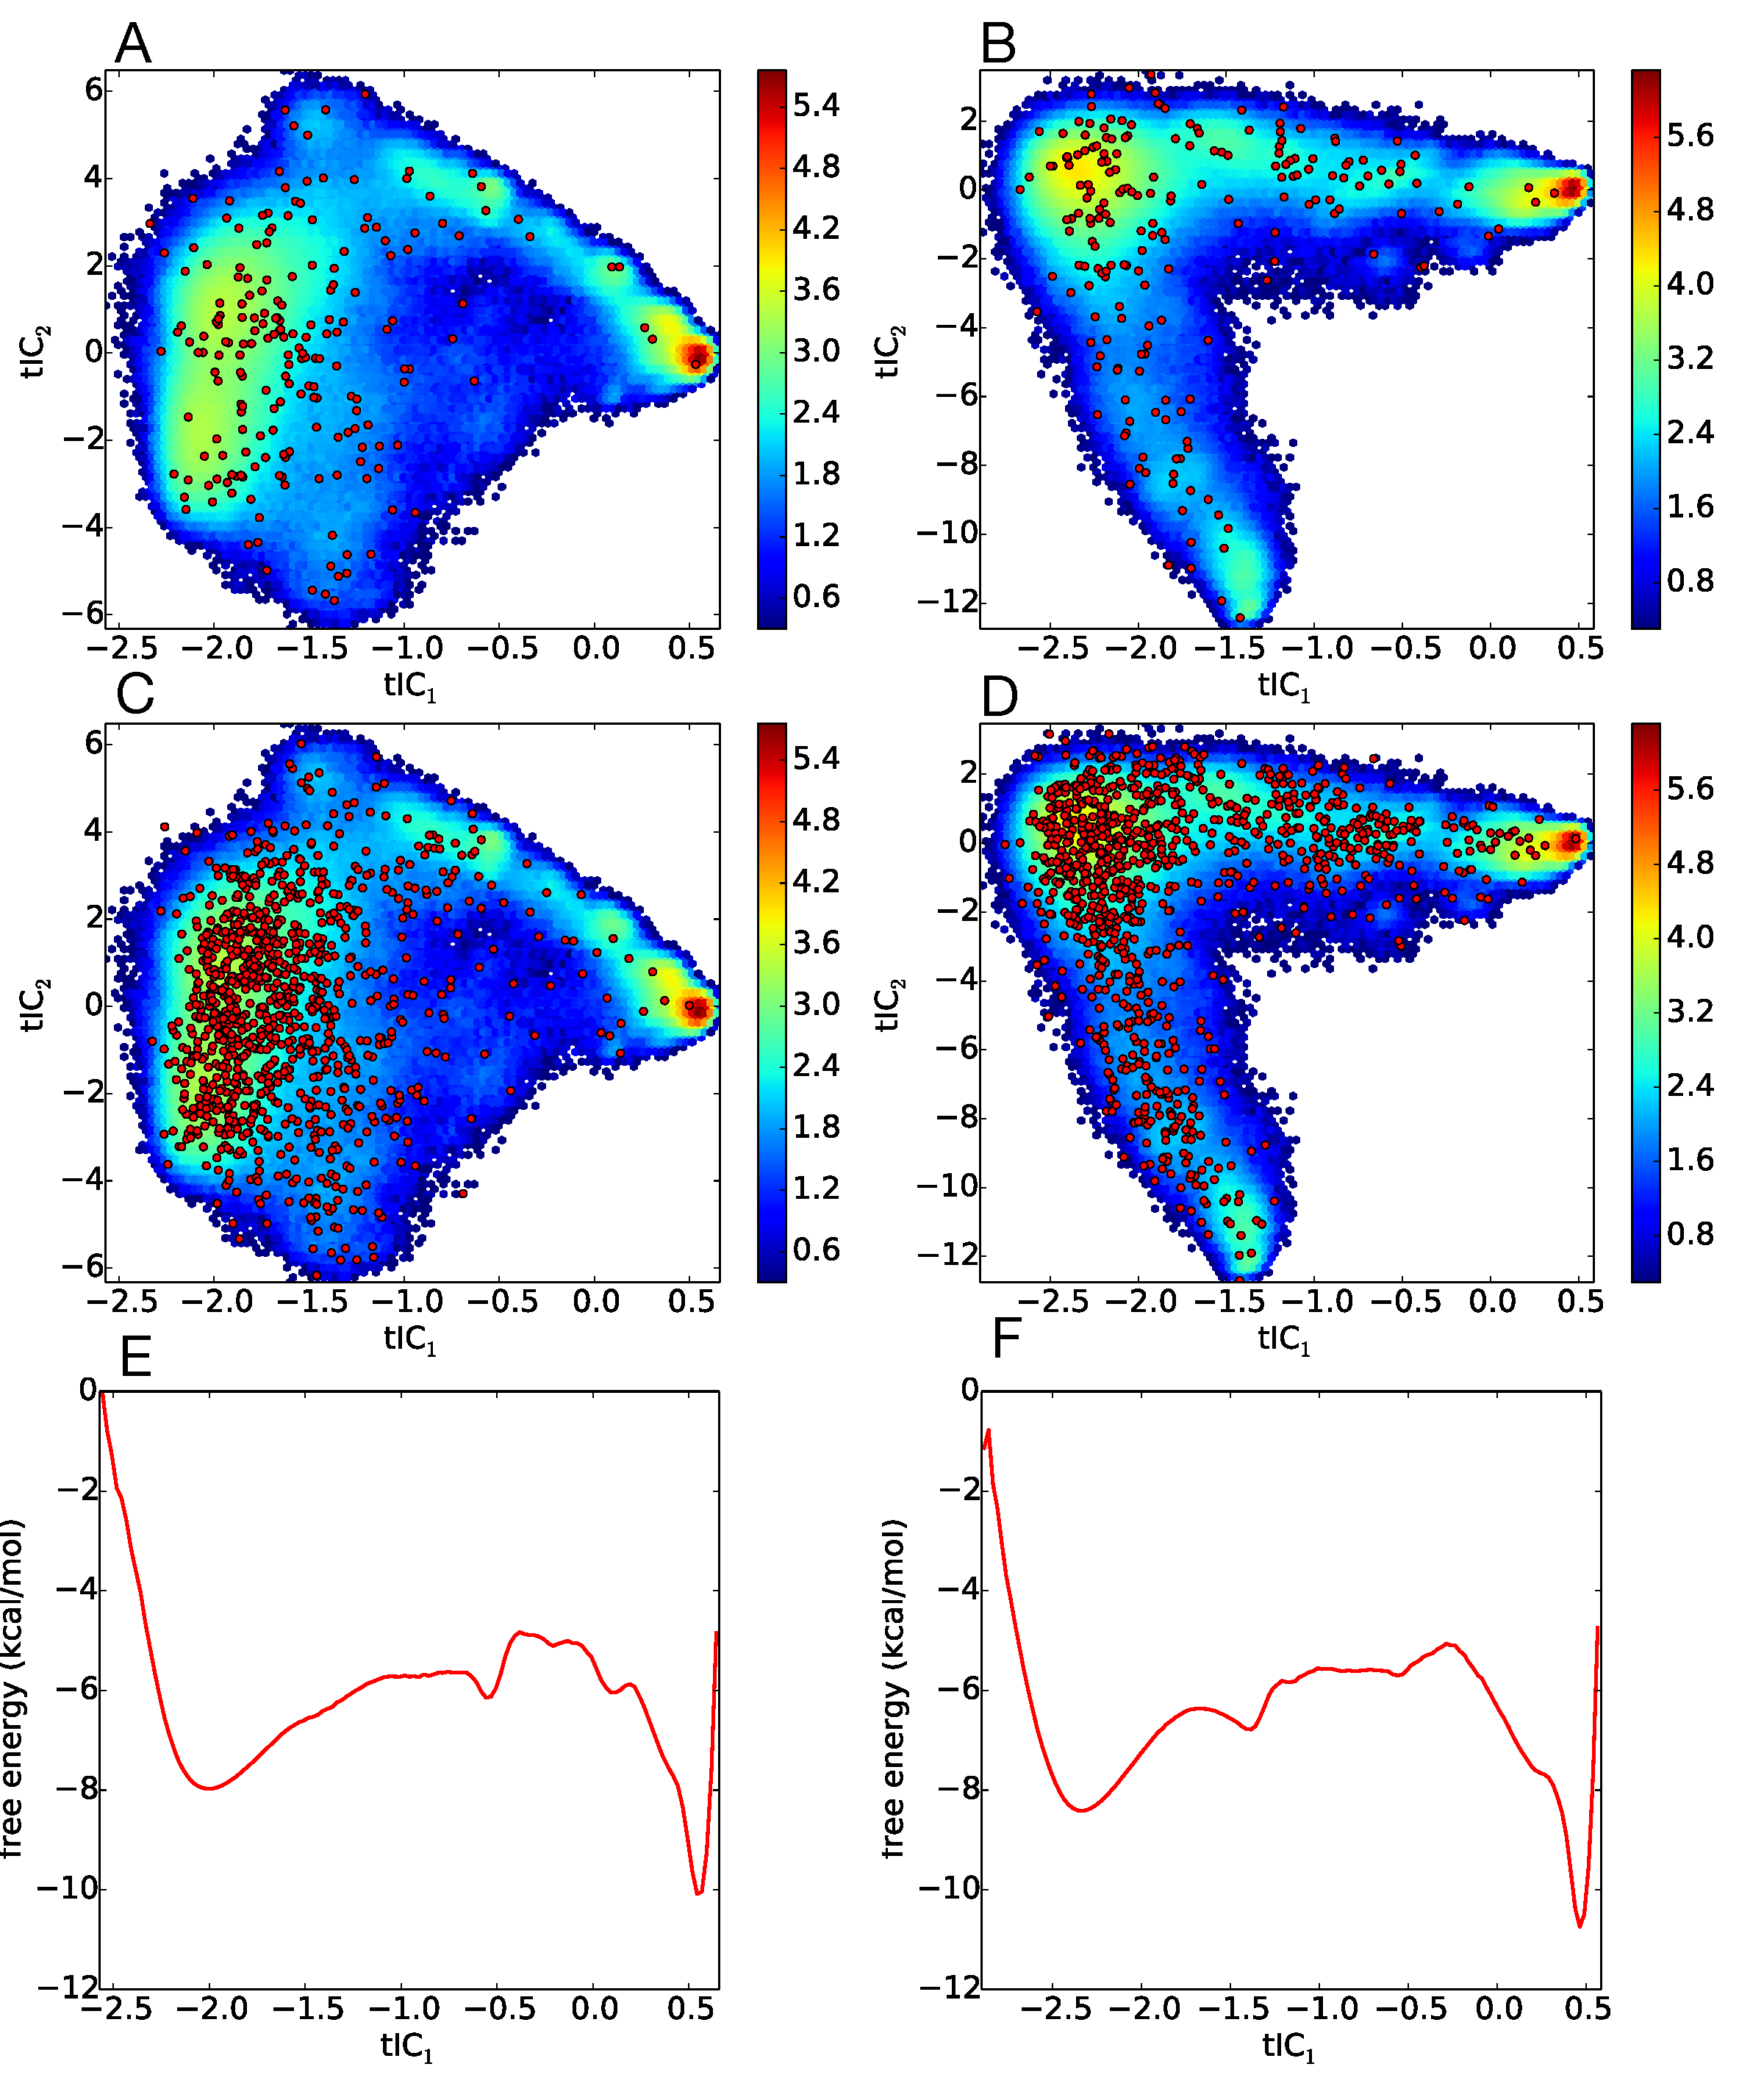
\includegraphics[width=0.8\paperwidth]{figures/tICA_subspace/tica_and_free_energy_GTT_NTL9.pdf}
\caption{Projection of GTT ((a) and (c)) and NTL9 ((b) and (d)) trajectory data onto the two largest tICA components, overlaid with the locations of the 200 and 1000 microstates respectively (red dots), and their free energy profiles calculated from the first tICA subspace with bin-width=0.025 unit.}
\end{figure*}





\section{Discussion}


The estimators approaches turned out that the folding time estimation from common MLE suffers greatly from doing seeding simulations; MLE with known populations incredibly rescued the relaxation time, but limited to use due to unknown equilibrium populations ahead of analysis; Row-normalized estimator could not always work with large lagtime in short seeding simulations, which obey the purposes of doing seeding simulations; MLE with population-weighted trajectory counts estimator also successfully improved the kinetics estimators and independent on the lengths of seeding trajectories. The potential applications of population-reweighted MLE on Markov State models are exciting. One application can be used to predict larger perturbation effects from different temperatures, force fields without running ultra-long simulations. However, the success of population-reweighted MLE is highly dependent on that perturbations won?t vary too much on the metastable state definitions.  Our method is similar to the weighted ensemble (WE), which each trajectory is assigned with a weight. However, WE mainly focus on pathway sampling where MSM can predict both kinetics and thermodynamics at the same time. Moreover, our approach is from a well-defined MSM, which all seeding simulations optimally can get converged faster. 

This idea--that both kinetic and thermodynamic information are necessary to obtain good MSMs--has motivated the development of multiensemble MSM estimators like DTRAM, TRAM, DHAM and DHAMed. These estimators combine both free energy estimation and MSM transition rate estimation, leveraging both thermodynamic and kinetic information from sampled trajectories to estimate an MSM.

All AIP journals require that the initial citation of
figures or tables be in numerical order.
\LaTeX's automatic numbering of floats is your friend here:
just put each \texttt{figure} environment immediately following 
its first reference (\verb+\ref+), as we have done in this example file. 

\begin{acknowledgments}
The authors thank the participants of Folding@home, without whom this work would not be possible.  We graciously acknowledge D. E. Shaw Research for providing access to the WW domain folding trajectory data. This research was supported in part by the National Science Foundation through major research instrumentation grant number CNS-09-58854 and National Institutes of Health grants 1R01GM123296-01 and NIH Research Resource Computer Cluster Grant S10-OD020095.
\end{acknowledgments}

%%%%% wide figure
\begin{figure*}
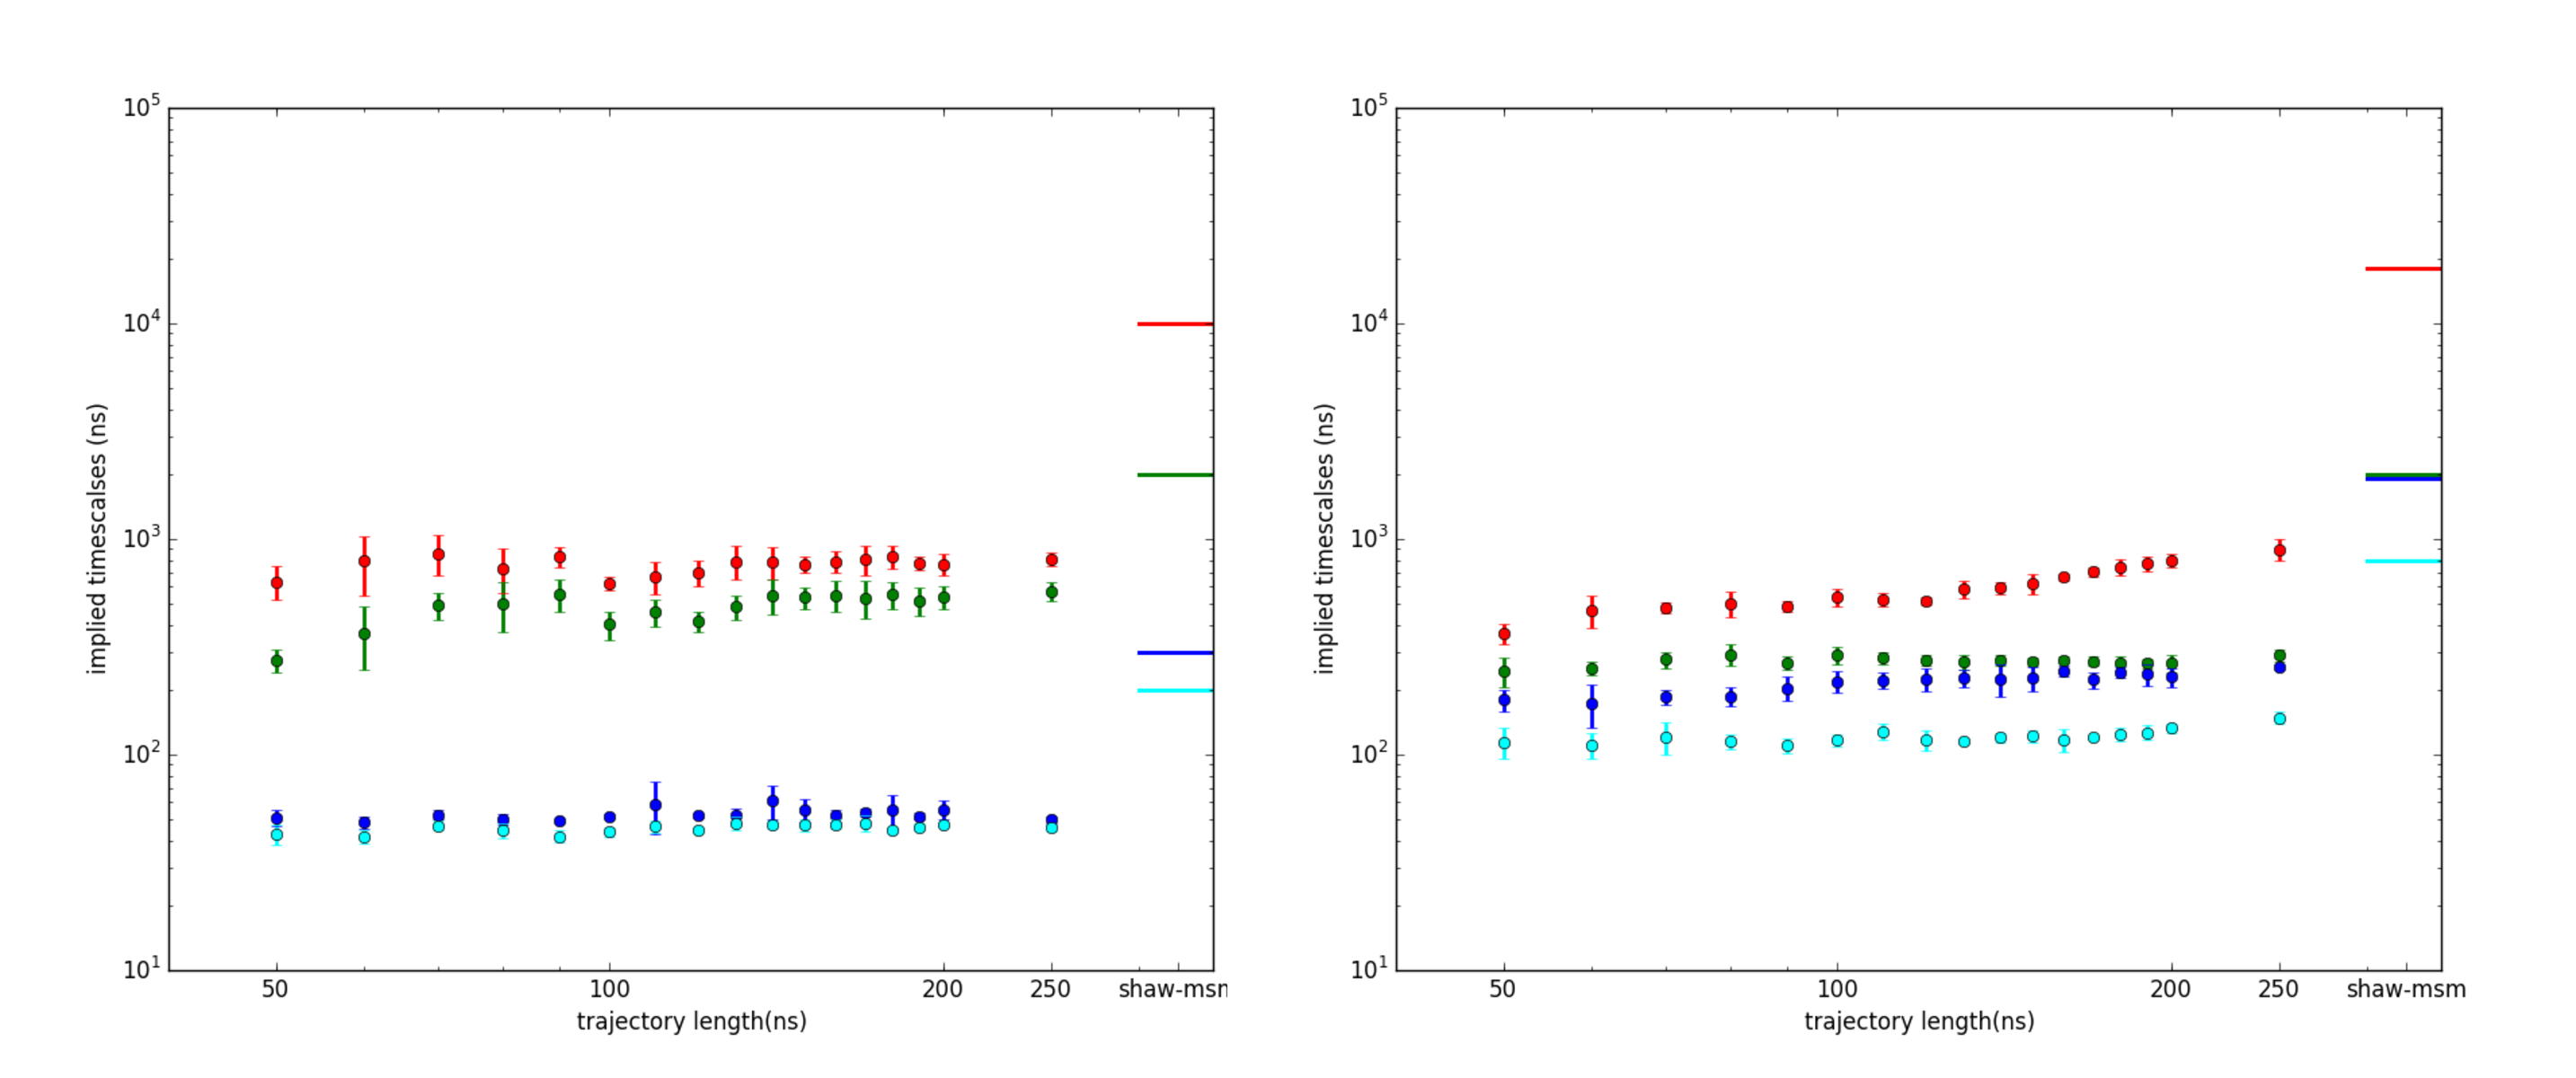
\includegraphics[width=0.8\paperwidth]{figures/NTL9_GTT/MLE_5trajs.pdf}% Here is how to import EPS art
\caption{Maximum-likelihood estimator (MLE) for both GTT(left) and NTL9(right) under-estimates implied timescales.}
\end{figure*}

\begin{figure*}
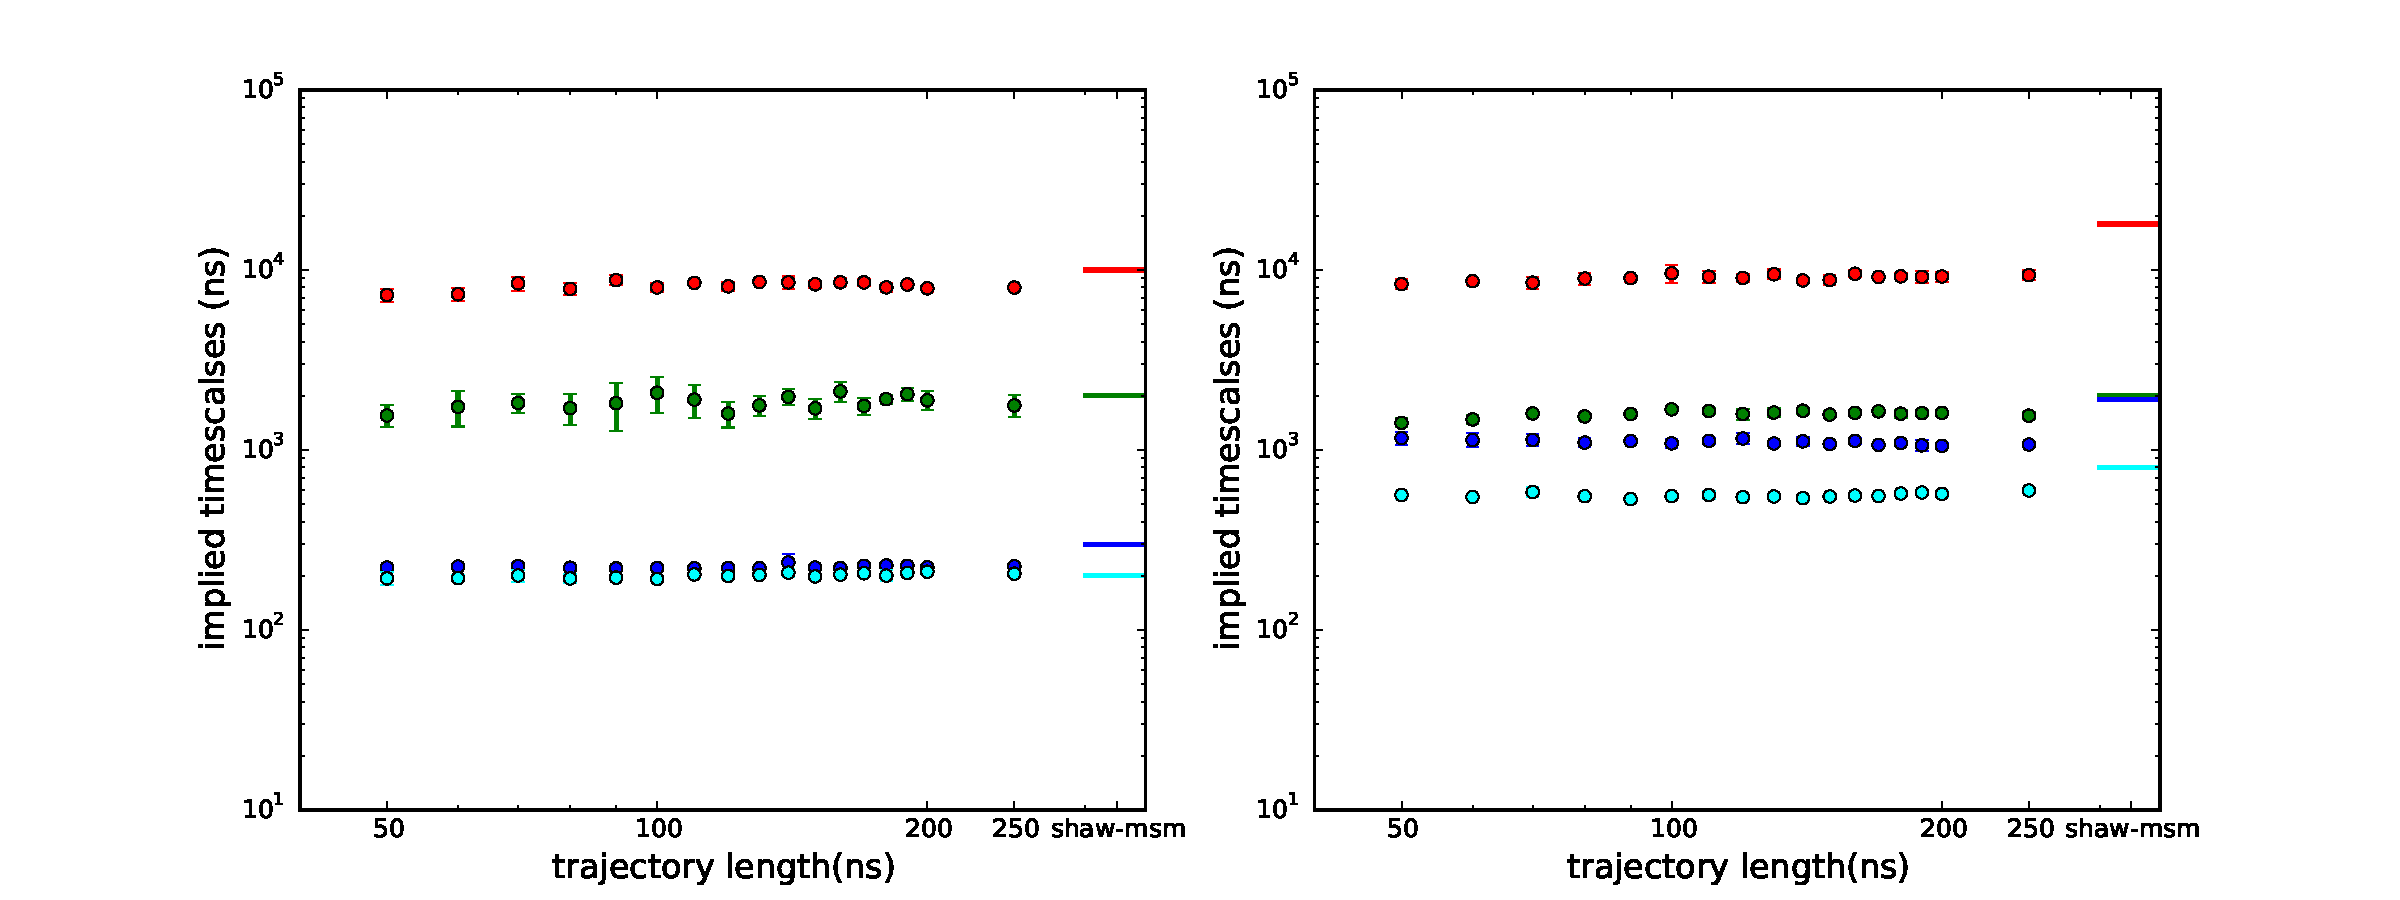
\includegraphics[width=0.8\paperwidth]{figures/NTL9_GTT/known_pop_5trajs.pdf}% Here is how to import EPS art
\caption{Maximum-likelihood estimator (MLE) with known populations estimator (MLE) for both GTT(left) and NTL9(right) well predicted implied timescales.}
\end{figure*}

\begin{figure*}
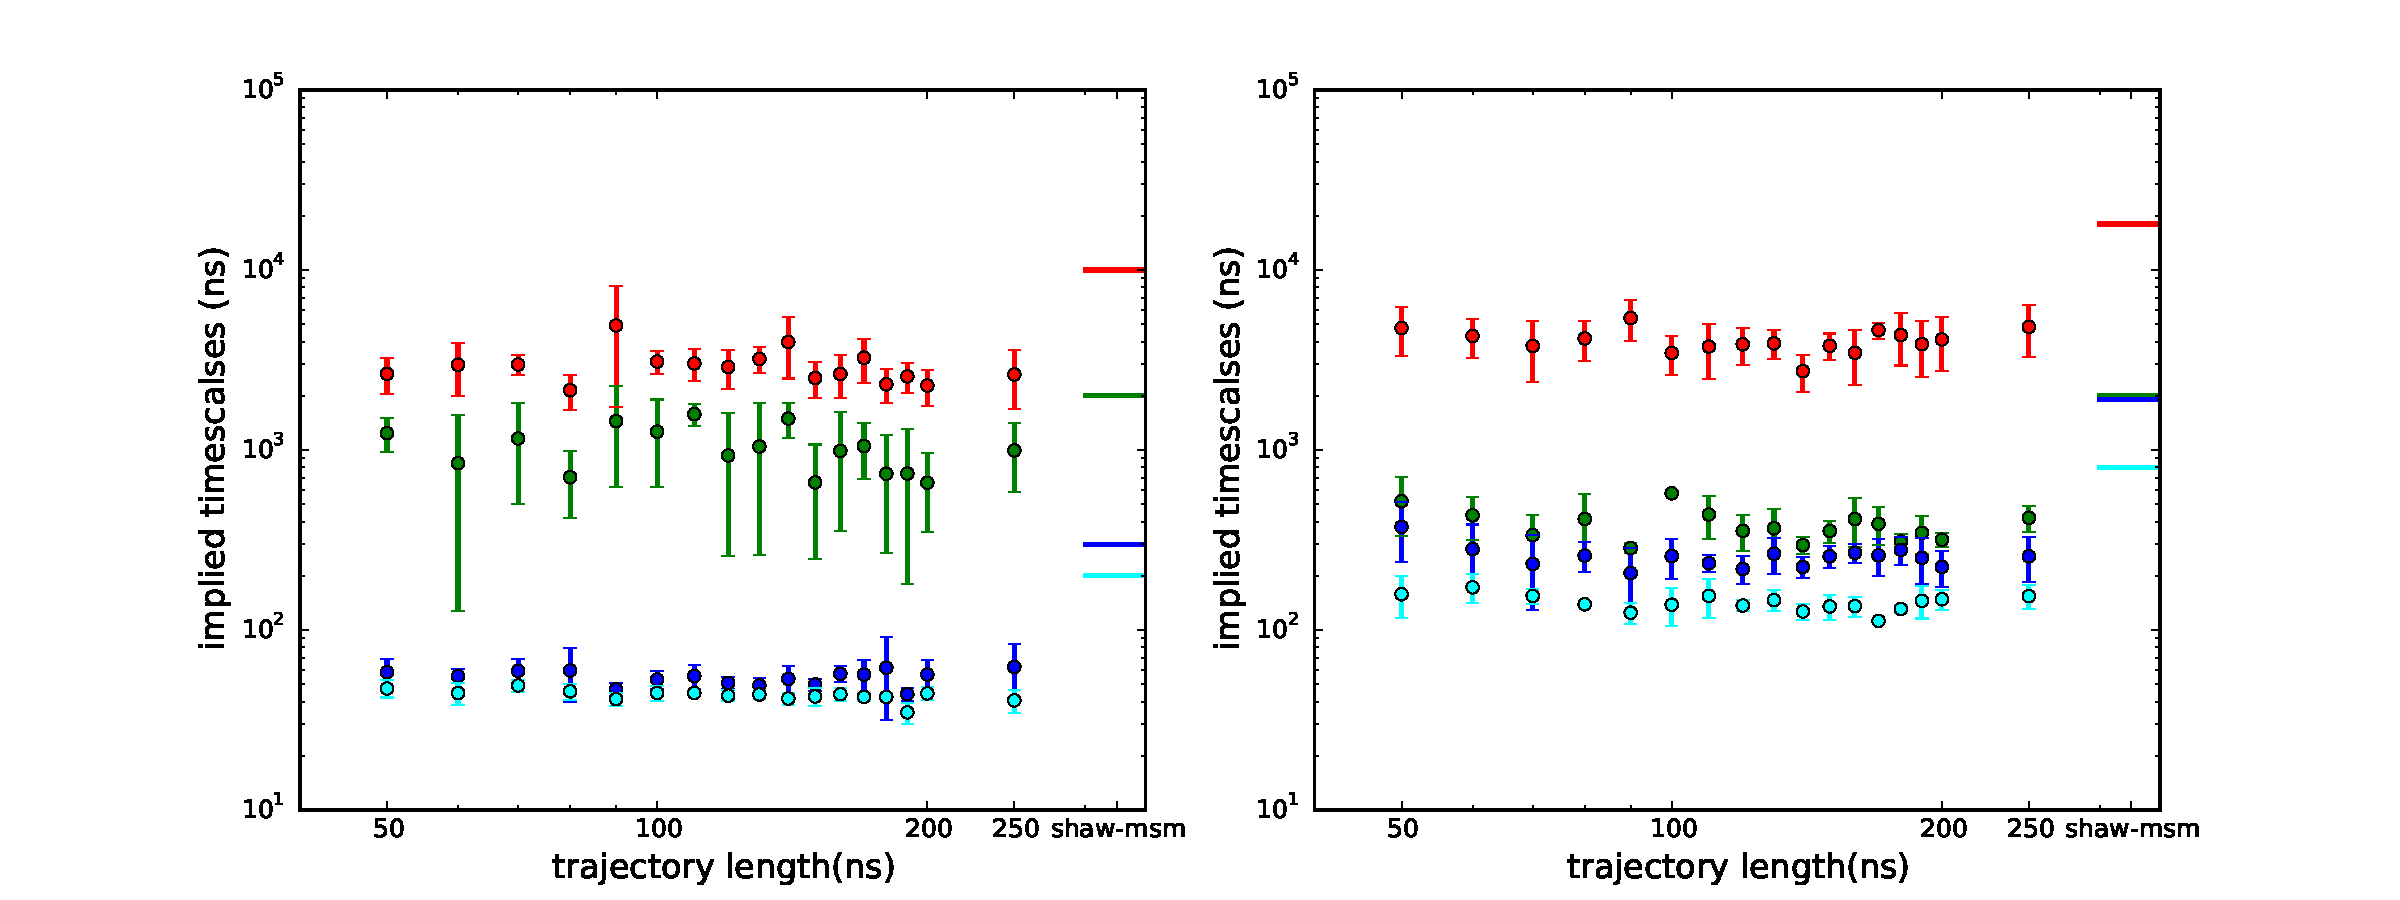
\includegraphics[width=0.8\paperwidth]{figures/NTL9_GTT/pop_reweighting_5trajs.pdf}% Here is how to import EPS art
\caption{Maximum-likelihood estimator (MLE) with population-weighted trajectory counts estimator (MLE) for both GTT(left) and NTL9(right) rescued implied timescales.}
\end{figure*}

\begin{figure*}
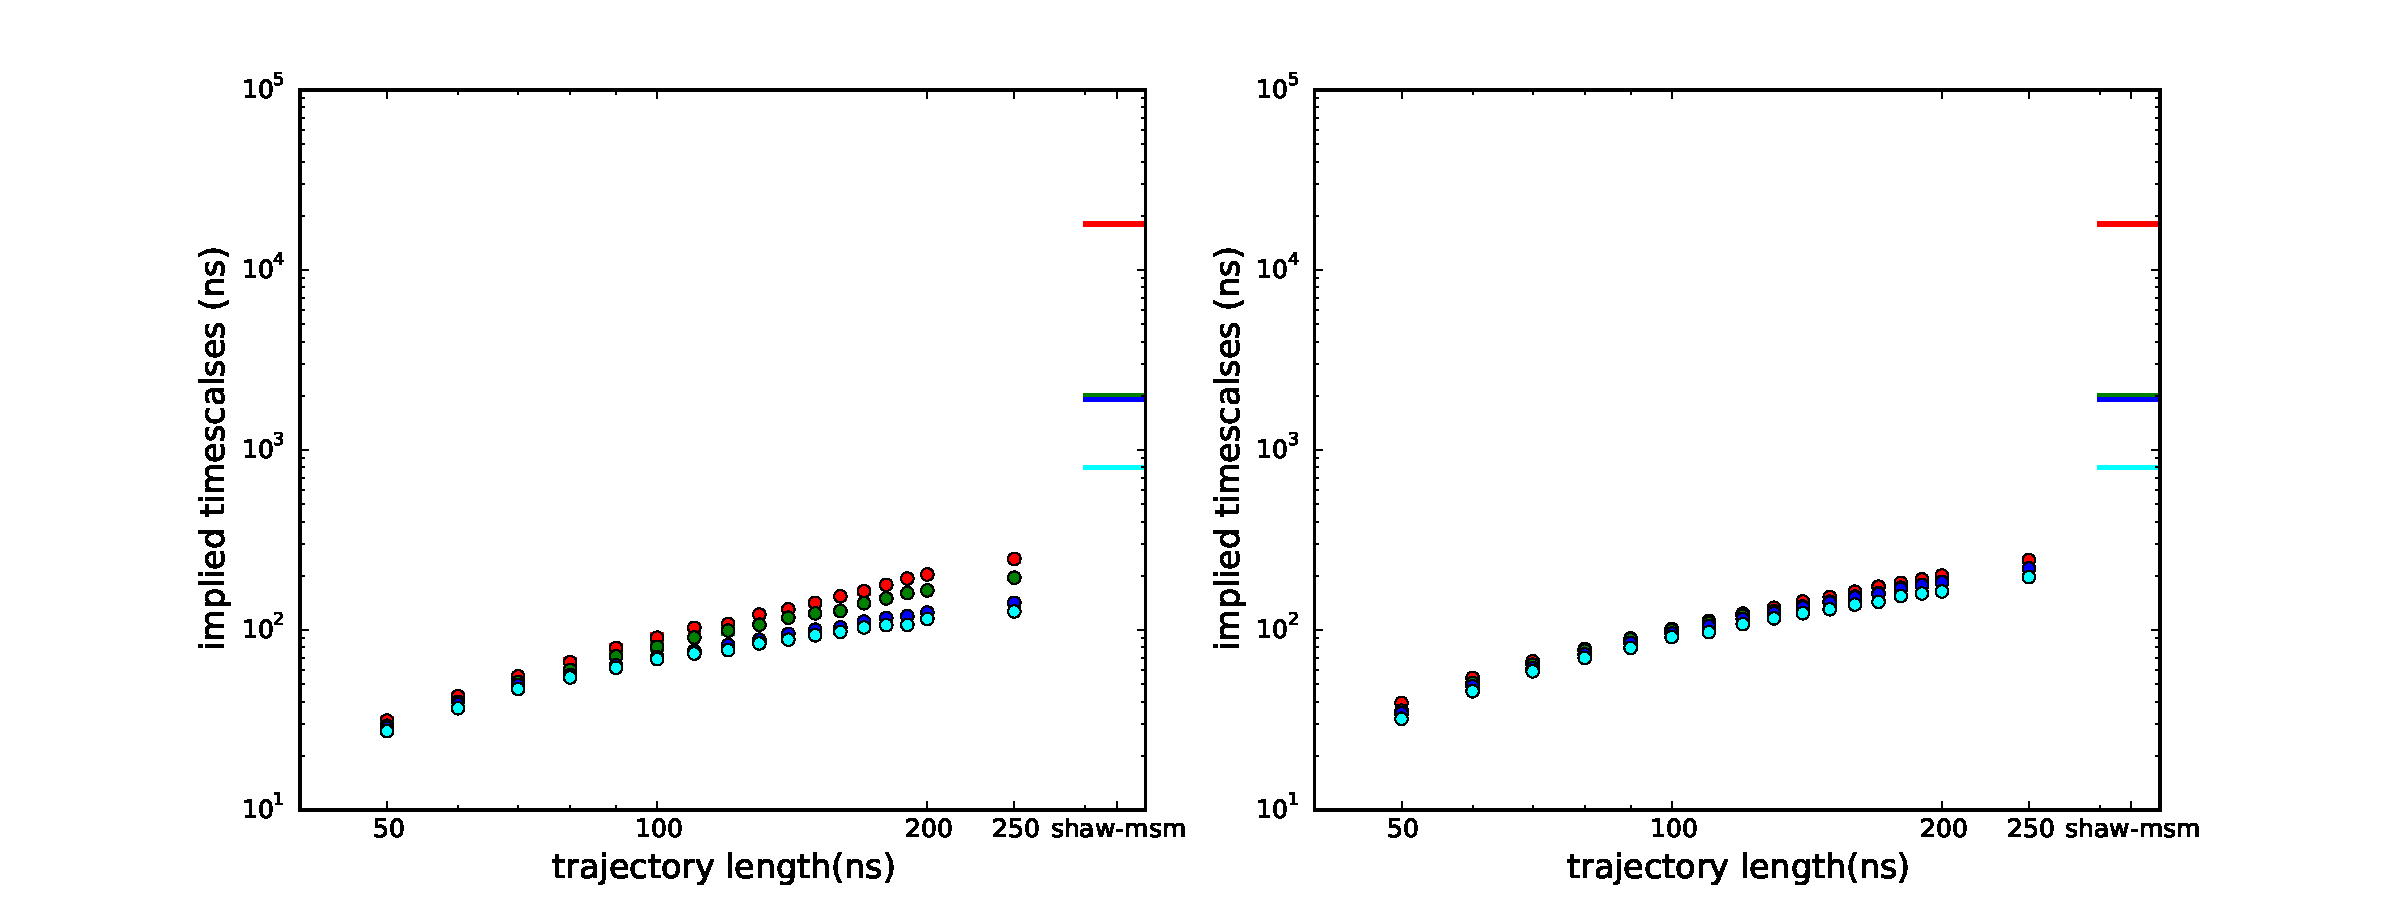
\includegraphics[width=0.8\paperwidth]{figures/NTL9_GTT/row_norm_5trajs.pdf}% Here is how to import EPS art
\caption{Row-normalized counts estimator for both GTT(left) and NTL9(right) badly predicted implied timescales.}
\end{figure*}

\begin{figure*}
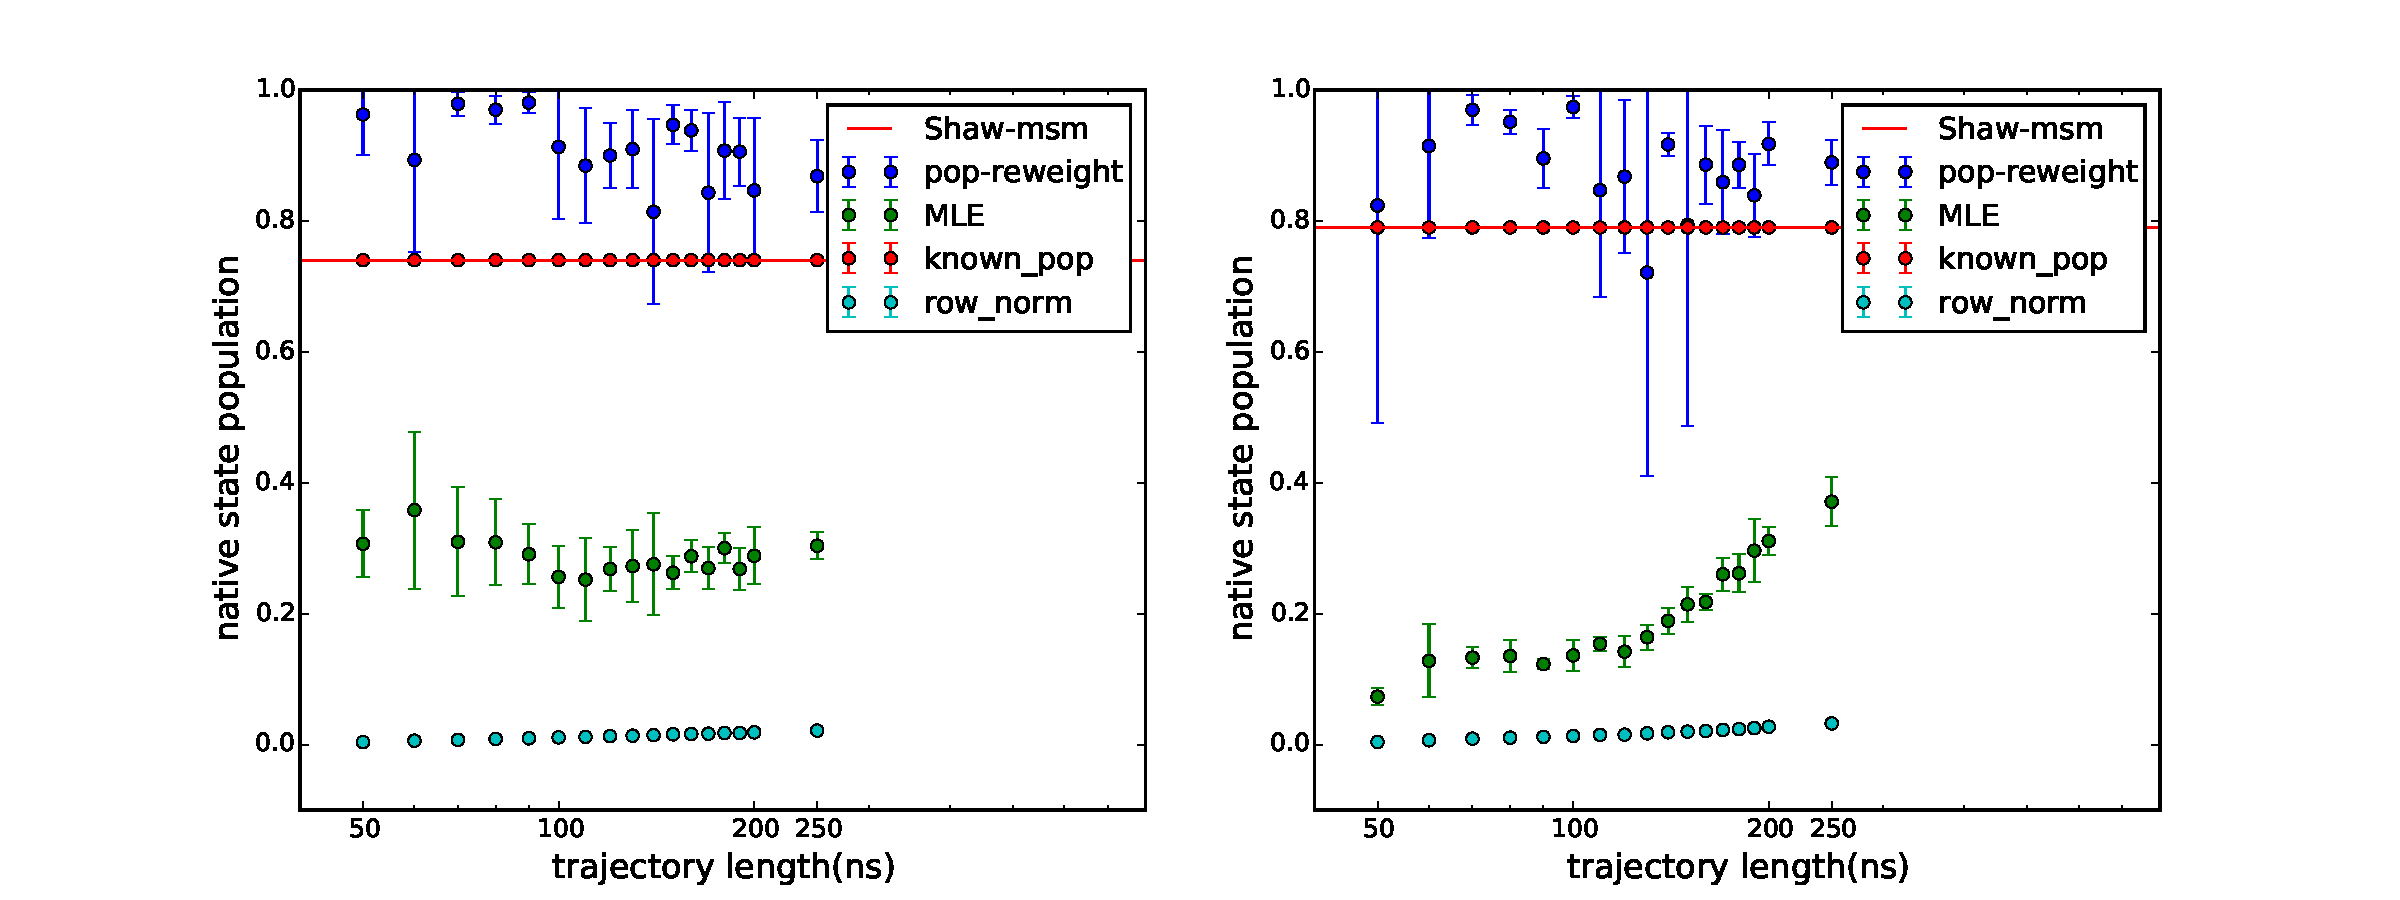
\includegraphics[width=0.8\paperwidth]{figures/NTL9_GTT/native_population_5trajs.pdf}% Here is how to import EPS art
\caption{The native state population  estimations of both GTT(left) and NTL9(right) with different estimators.}
\end{figure*}


%
% ****** End of file aipsamp.tex ******

\section{Bullet points}

\subsection{The accuracy of different estimators on seeding data from GTT and NTL9}

In general, for this kind of seeding data, row-normalized counts work poorly in estimating both timescales and native populations.  MLE does better at estimating timescales, but not native populations.  The two methods that ``rescue'' the native populations (by properly weighting the contributions of counts) are MLE-known-pi  and population reweighting.  By definition. the known-pi constraints the populations, while pop-reweighted has a lot of potential errors, but estimate values in the right range.

What about OOM and corrected timescales?  Our results suggest that these methods don't work particularly well with short re-seedin data.   The OOM timescales are pretty good, but the native populations are very bad.  Furthermore, the practical application of OOM methods are limited by the number of states, simply due to the $O(N^3)$  scaling of the algorithm limits the calculation for the all-atom models to 200 states.

When we are able to increase the number of states in the all-atom model to 1000 state,both the timescales and the populations are much better, and furthermore, we can get good estimates form much shorted trajectory lengths (smaller than the complete 1 ms data set)

Lastly, we can use the populations of GTT to reweight a mutant srquence, Fip35, and get pretty good est,ates of the slower rate of this folder.

% \nocite{*}
\bibliography{seeding}% Produces the bibliography via BibTeX.

\end{document}